% Chapter Template

\chapter{2-D Memristor Simulation} % Main chapter title

\label{Chapter6} % Change X to a consecutive number; for referencing this chapter elsewhere, use \ref{ChapterX}

\lhead{Chapter 6. \emph{Memristor Simulation}} % Change X to a consecutive number; this is for the header on each page - perhaps a shortened title

Even though 1-D simulation was able to capture the main characteristics of the memristor it is still lacking certain physical effects that can be captured in a 2-D simulation such as the movement of ions inside the electrolytic solution which cancels some applied electric field. This chapter shows the simulation of a memristor in 2-D and compares the results with 1-D simulations. It starts with the simulation of a memristor with different PEDOT:PSS layer thicknesses and shows the changes in particle distributions, electric field and current density. 
Transient simulations with a pulse train and a sinusoidal potentials are presented and compared to 1-D siumlations. Finally current vs time and I-V curves for an actual memristor is used to show the accuracy of 2-D simulations in capturing the behavior of the actual device .  

\section{Effect of PEDOT:PSS Thickness}

The physical dimensions of the memristor was presented in the previous chapter. Thickness of the PEDOT:PSS layer is very small compared to the other dimensions of the device such as the thickness of the electrolyte and length of the conductive material. This complicates the simulation of the PEDOT:PSS strip using a uniform mesh. Although non uniform meshing seems like an appropriate solution an examination of the numerical limitations show that this is not the case. Decreasing the mesh size in one dimension severely reduces the maximum time step size for the entire simulation therefore non uniform meshing is not an appropriate solution for this problem. 

An alternative solution to this meshing problem is using an infinitesimally thin PEDOT:PSS layer in a 2-D simulation. This method is used for the memristor simulations in this chapter. For PEDOT:PSS effects in 2-D are ignored since the layer thickness is 10000 times smaller than other dimensions such as the thickness of the electrolyte. For holes in the conductive layer only the horizontal component of the electric field is used and all the current densities are calculated in 1-D. Following plots compare two simulations with PEDOT:PSS thicknesses higher than the actual device and a 2-D simulation with 1-D PEDOT:PSS layer.  

The memristor was simulated using a constant potential at the contacts. Left metal contact is kept at 1 V and the right metal contact is grounded. Resistivity measured at the right contact for different PEDOT:PSS thicknesses is shown in figure \ref{thick_resistivity}. Resistivity plots show as the thickness gets smaller the device responds faster. This is due to the decrease in the distance lithium ions have to travel inside PEDOT:PSS in order to change its resistivity. Another change in the behavior of the memristor is its resistivity at steady state. The increase in resistivity for different thicknesses at steady state can be attributed to the ion/hole interaction at the interface between PEDOT:PSS and electrolyte solution which is illustrated in the following figures \ref{thick_p_ss}, \ref{thick_li_ss} and \ref{thick_perch_ss}. \textbf{(not sure about this)}

\begin{figure}[!htp]
\centering
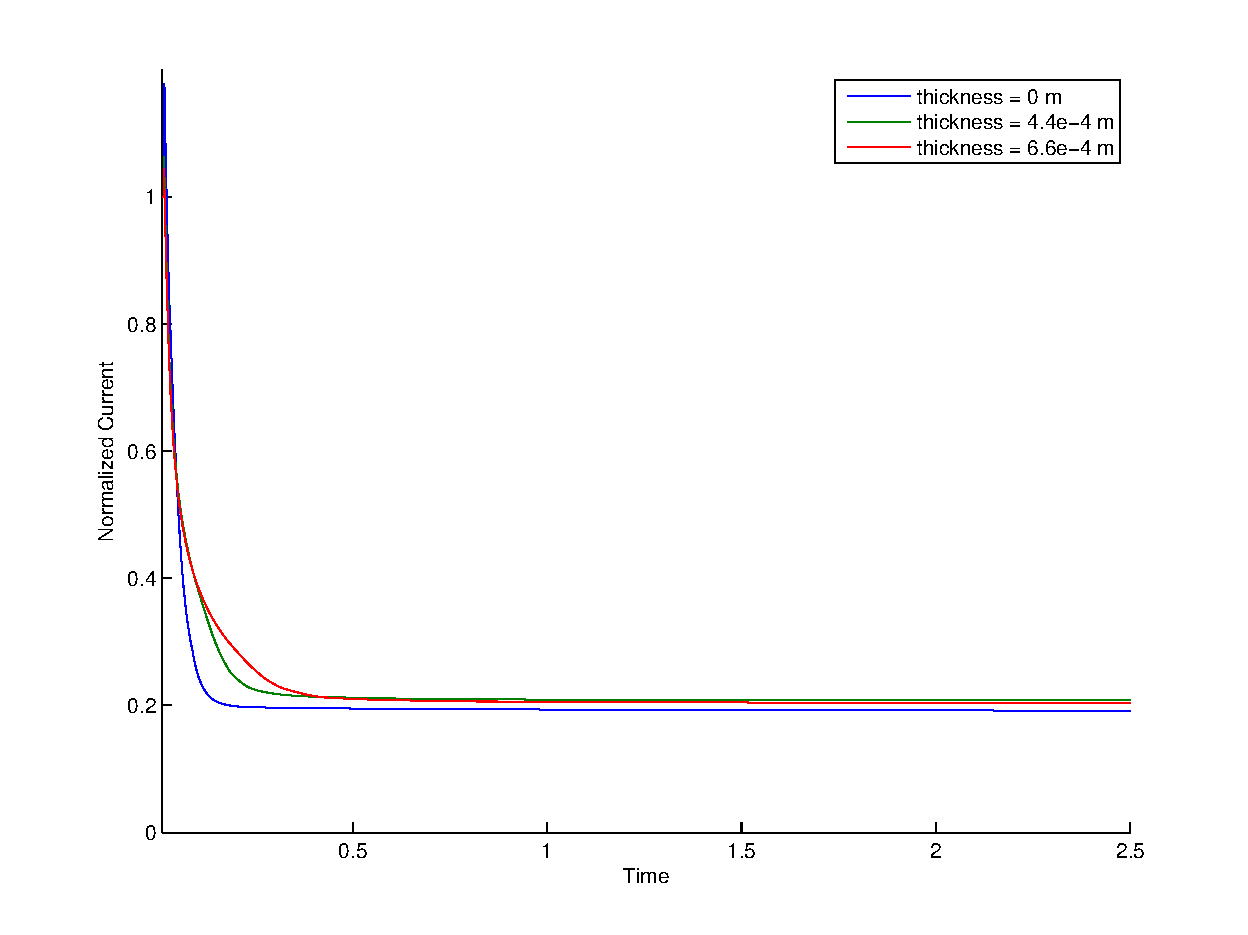
\includegraphics[scale=0.50]{2D_Memristor_Thick_Resistivity}
\caption{} 
\label{thick_resistivity}
\end{figure}

Figure \ref{thick_p_ss} shows hole distribution in PEDOT:PSS at steady state for different thicknesses. The electrolyte is on top of PEDOT:PSS but it is not visible in these plots since its hole concentration is zero at all times but they do affect the distribution of holes. As lithium ions move into the PEDOT:PSS they move towards the negative contact and pushes the holes out. This effect can be seen in figures \ref{thick_p_ss} and  \ref{thick_li_ss}. For all thicknesses there is a section of the hole density which is missing due to lithium ions.

The accumulation of holes at the surface of the PEDOT:PSS is due to perchlorate ions accumulating near the positive contact in the electrolyte (figure \ref{thick_perch_ss}). As perchlorate ions accumulate to cancel the electric field they also attract holes towards the surface.
\begin{figure}[!htp]
\centering
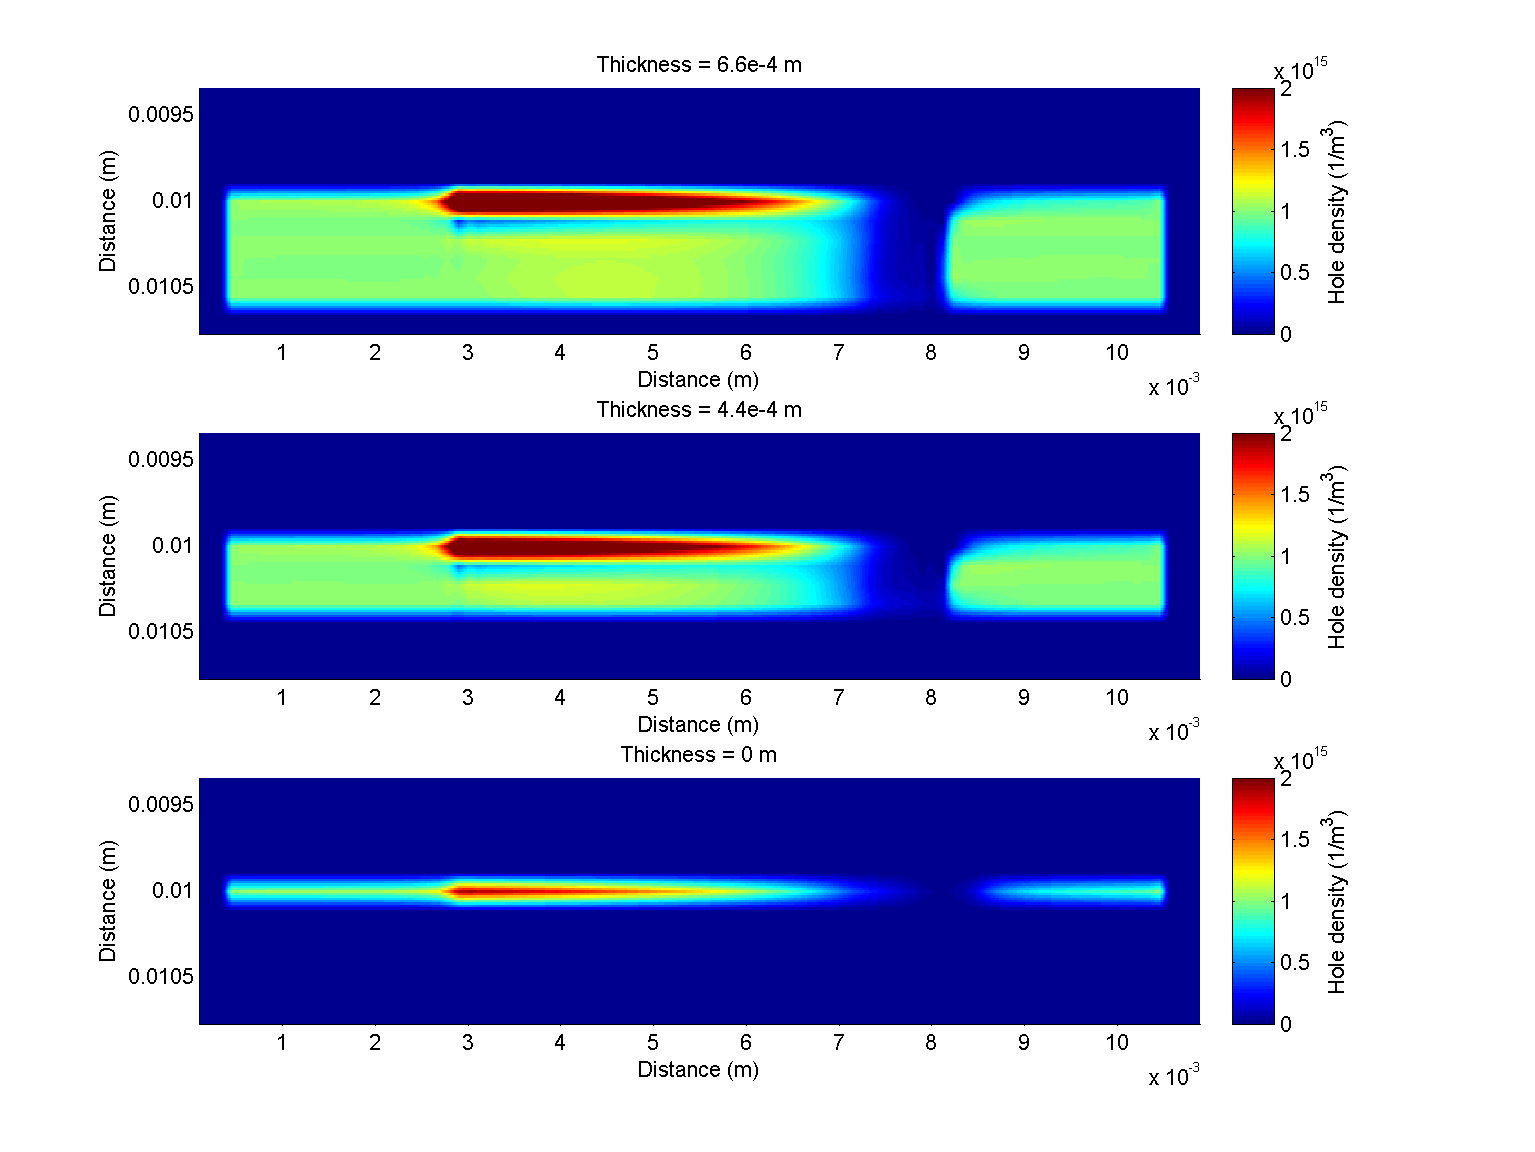
\includegraphics[scale=0.50]{2D_Memristor_Thick_Hole_SS}
\caption{} 
\label{thick_p_ss}
\end{figure}

\begin{figure}[!htp]
\centering
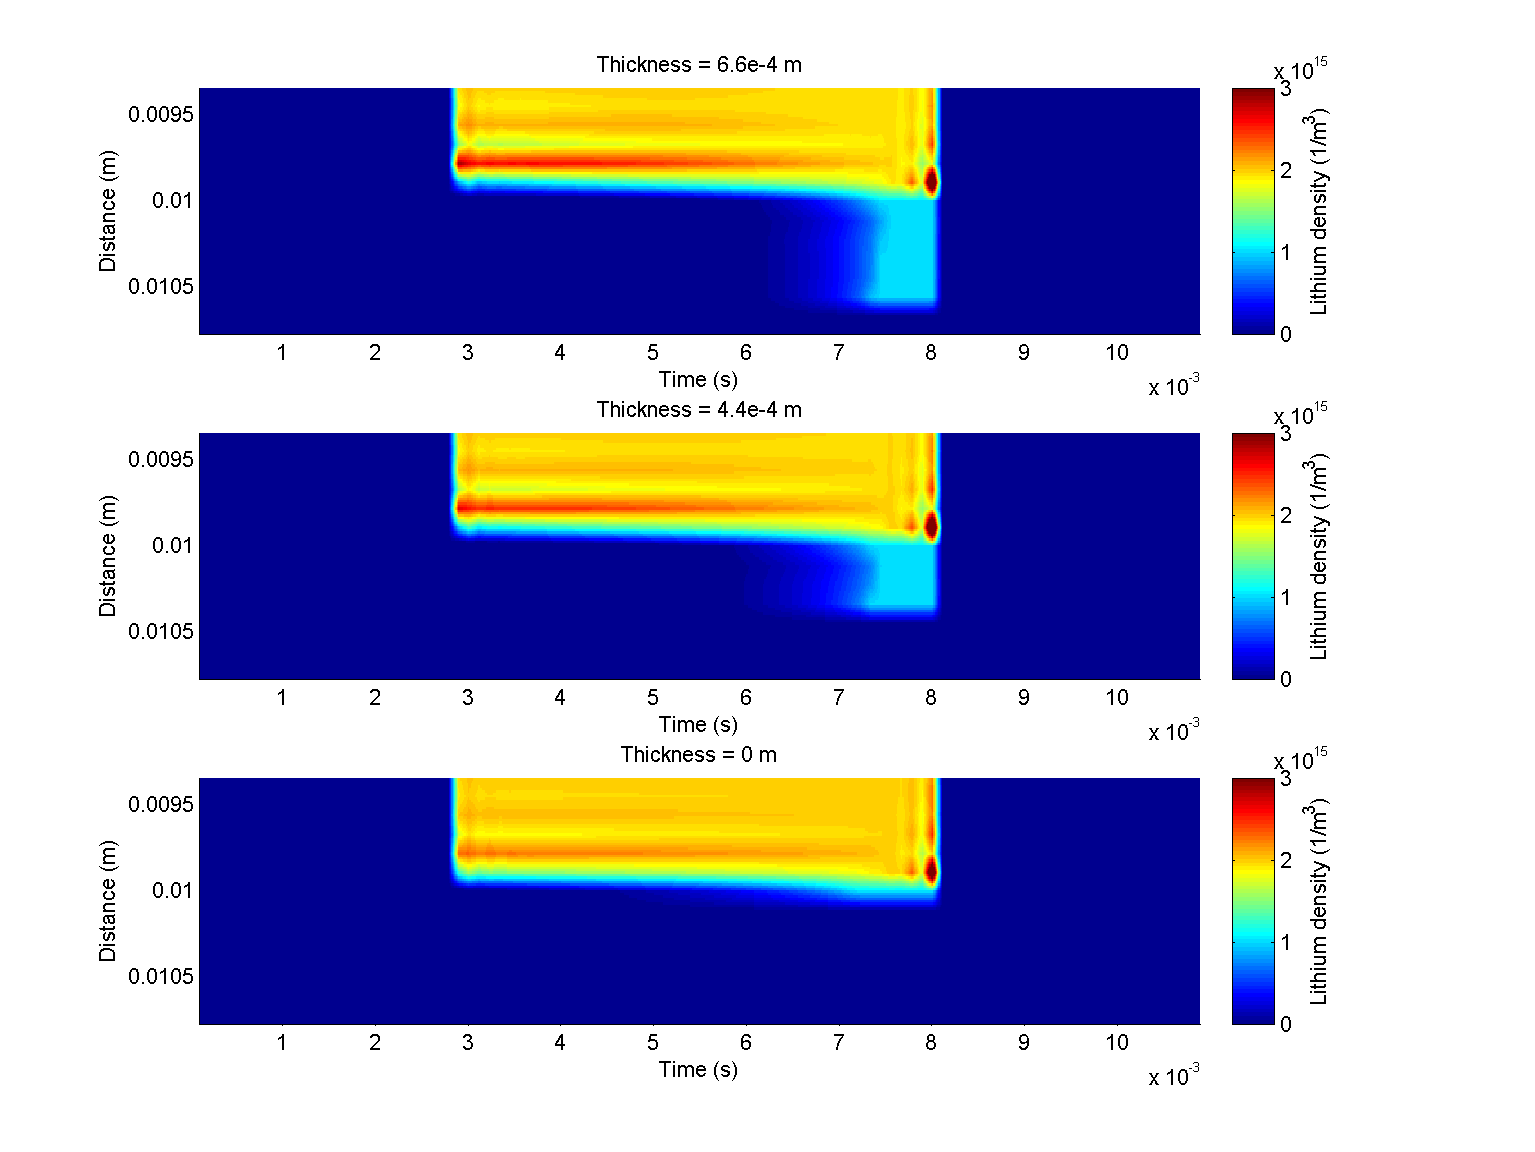
\includegraphics[scale=0.50]{2D_Memristor_Thick_Lithium_SS}
\caption{} 
\label{thick_li_ss}
\end{figure}

\begin{figure}[!htp]
\centering
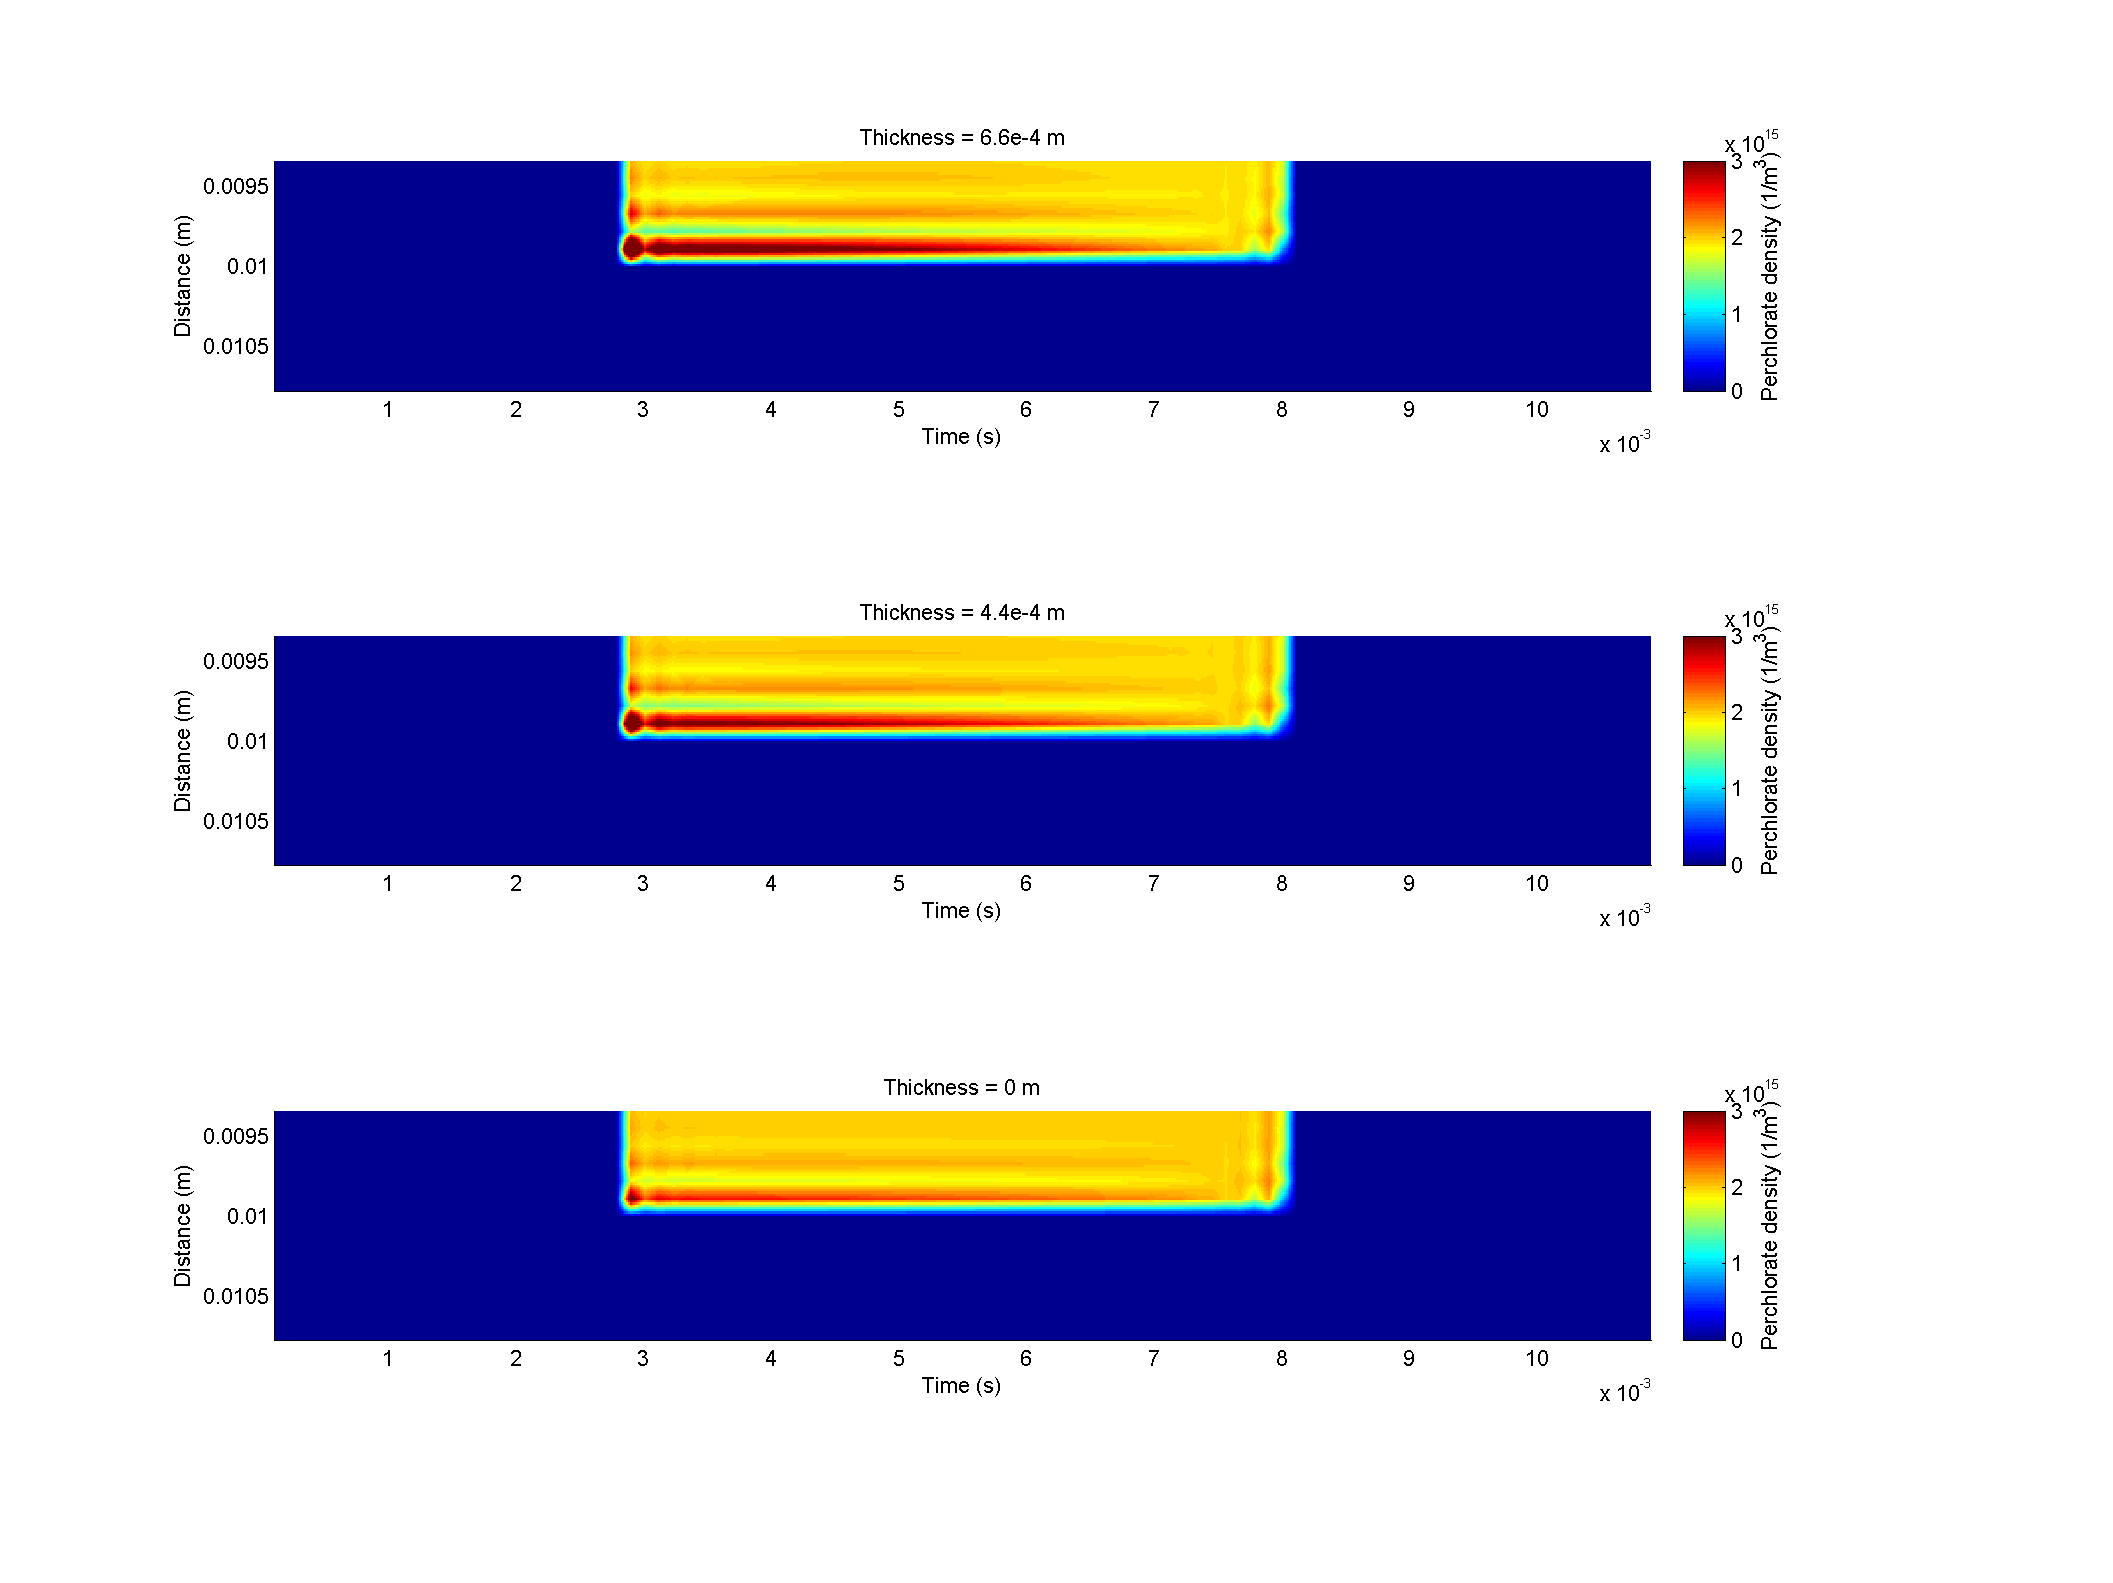
\includegraphics[scale=0.40]{2D_Memristor_Thick_Perchlorate_SS}
\caption{} 
\label{thick_perch_ss}
\end{figure}

\clearpage
Figure \ref{thick_netq_p} shows the hole charge density at the surface of the PEDOT:PSS and net charge density in the electrolyte near PEDOT:PSS. Again negative charges that accumulate on the left side of the electrolyte attract holes and positive charges on the right side push them out. This additional mechanism is the key difference between 1-D and 2-D simulations. In 1-D simulation, ion density inside the electrolyte and the changes in the electric field due to these charges were not present.

\begin{figure}[!htp]
\centering
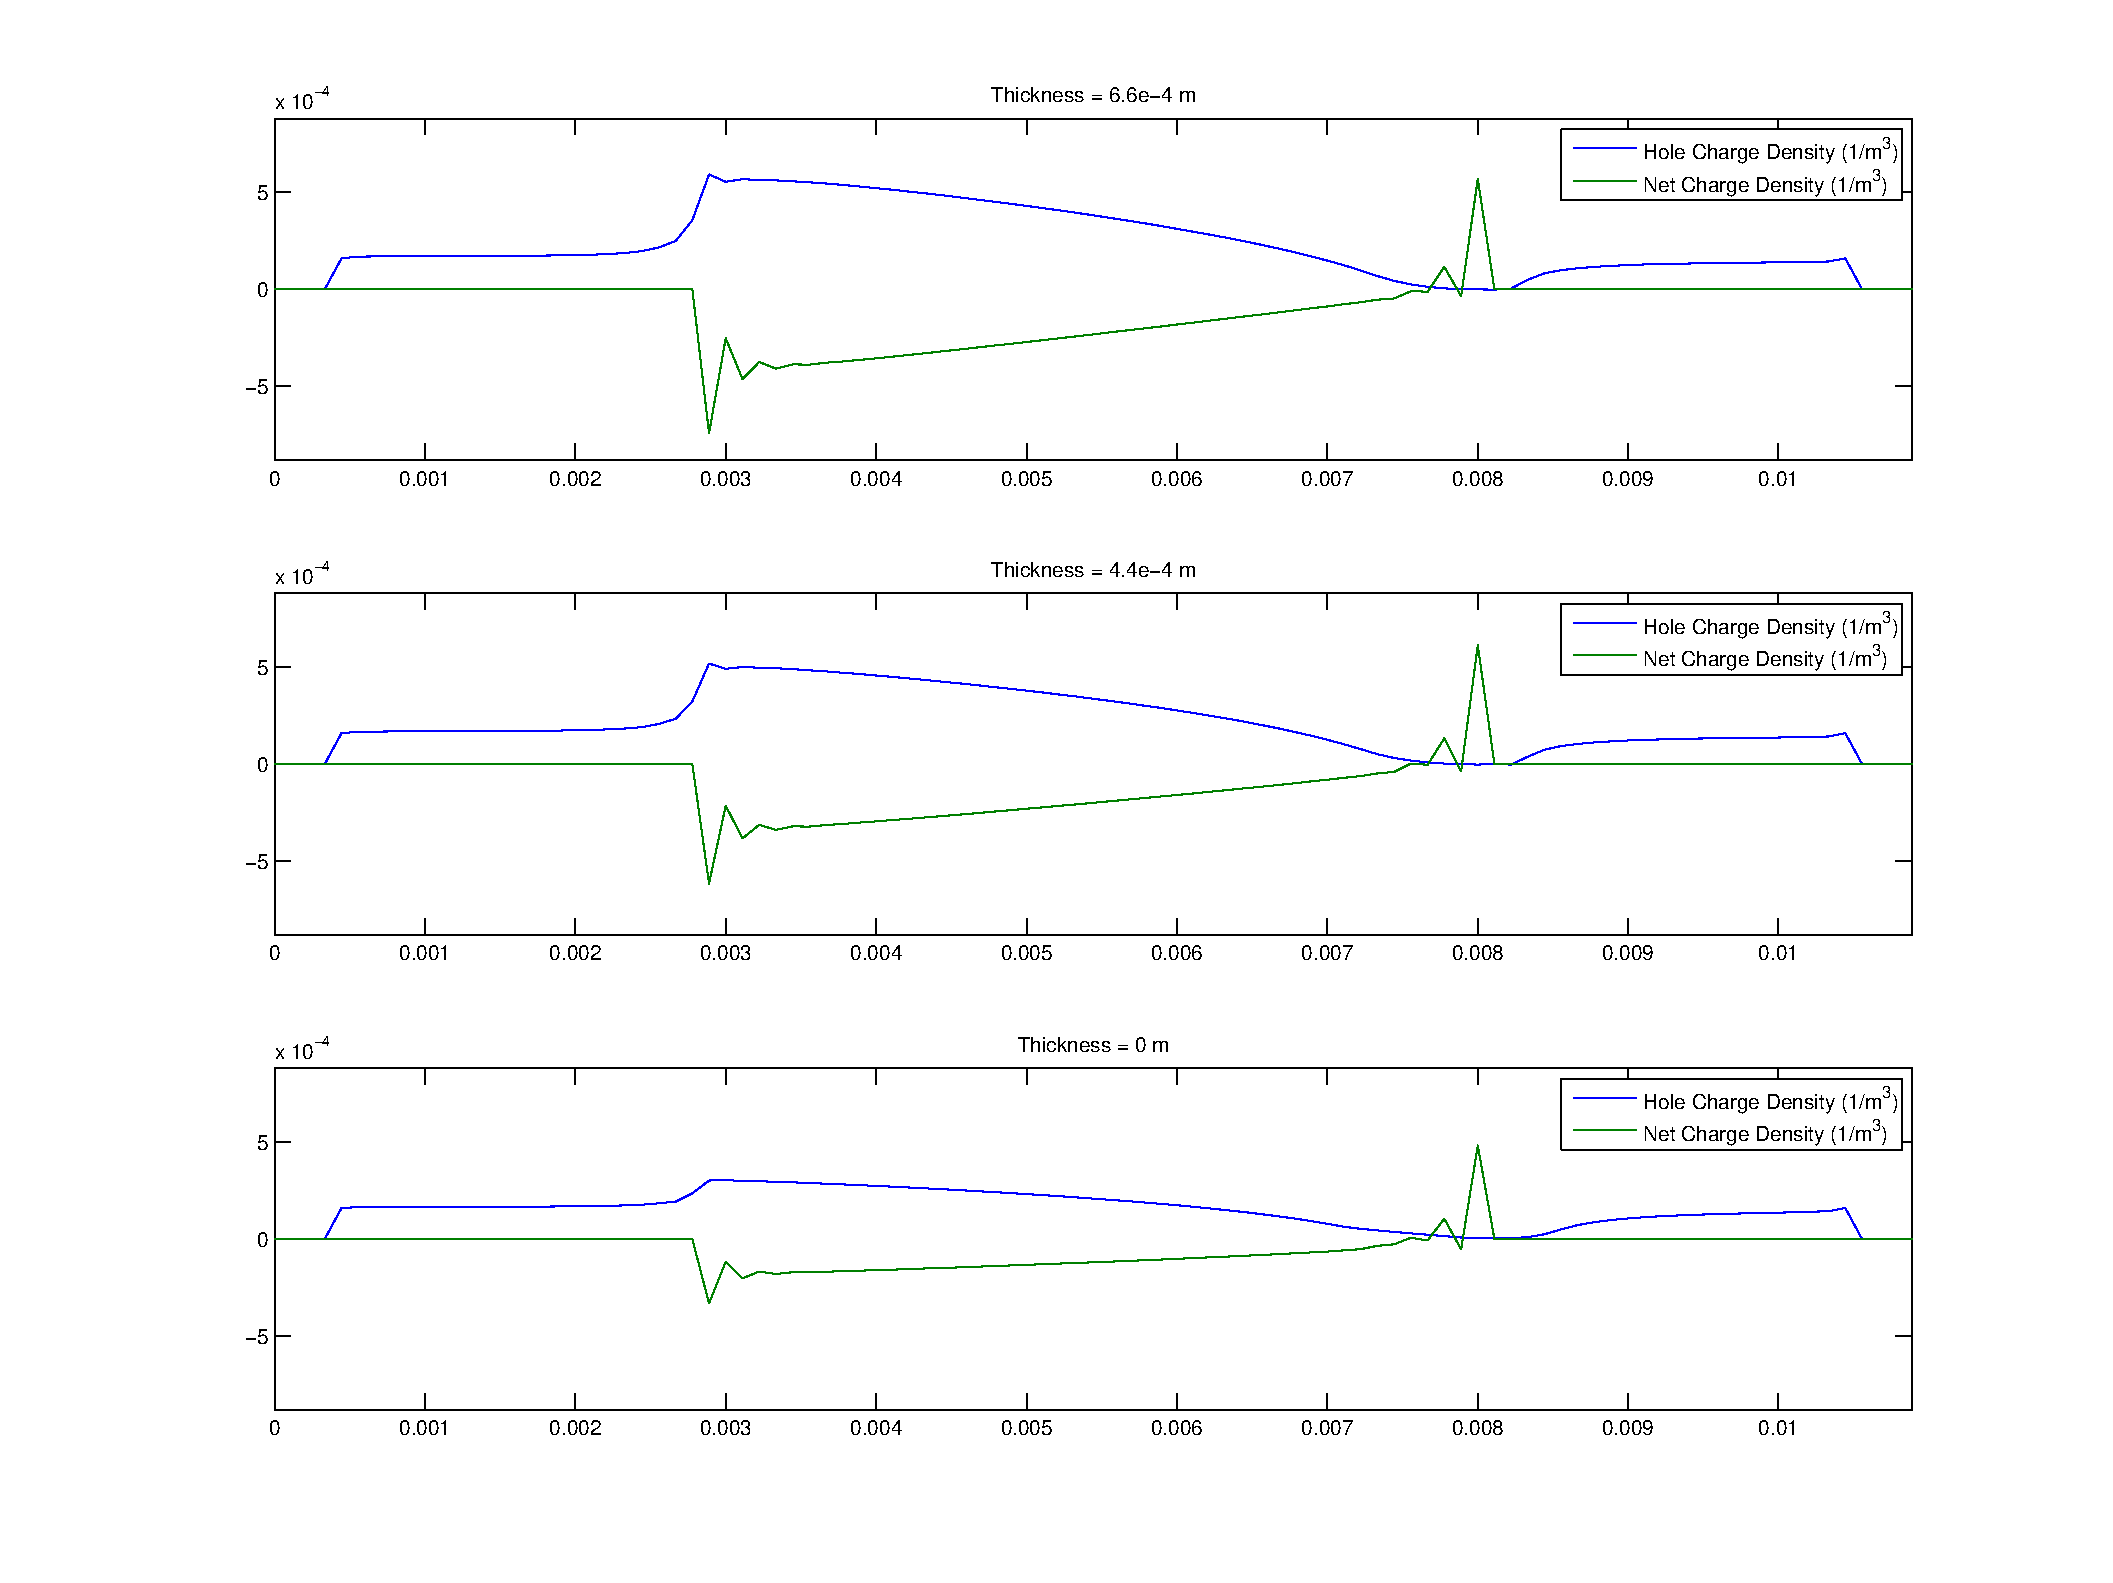
\includegraphics[scale=0.40]{2D_Memristor_netq_hole}
\caption{} 
\label{thick_netq_p}
\end{figure}

As shown in the previous chapter, electric field has the highest value where lithium ions accumulate. Figure \ref{thick_efield} shows the change in the accumulation of the electric field as PEDOT:PSS gets thinner. For all thicknesses most of the potential drop occurs where lithium ions accumulate and it is concentrated at the surface of the PEDOT:PSS. 

Above plots showed that changing the thickness of the PEDOT:PSS does not have a drastic effect in the operation of the memristor since most of the changes occur at the interface between electrolyte and PEDOT:PSS. 1-D approximation the polymer conductor contains all the necessary physics for the simulation of the memristor described in chapter 5.

\begin{figure}[!htp]
\centering
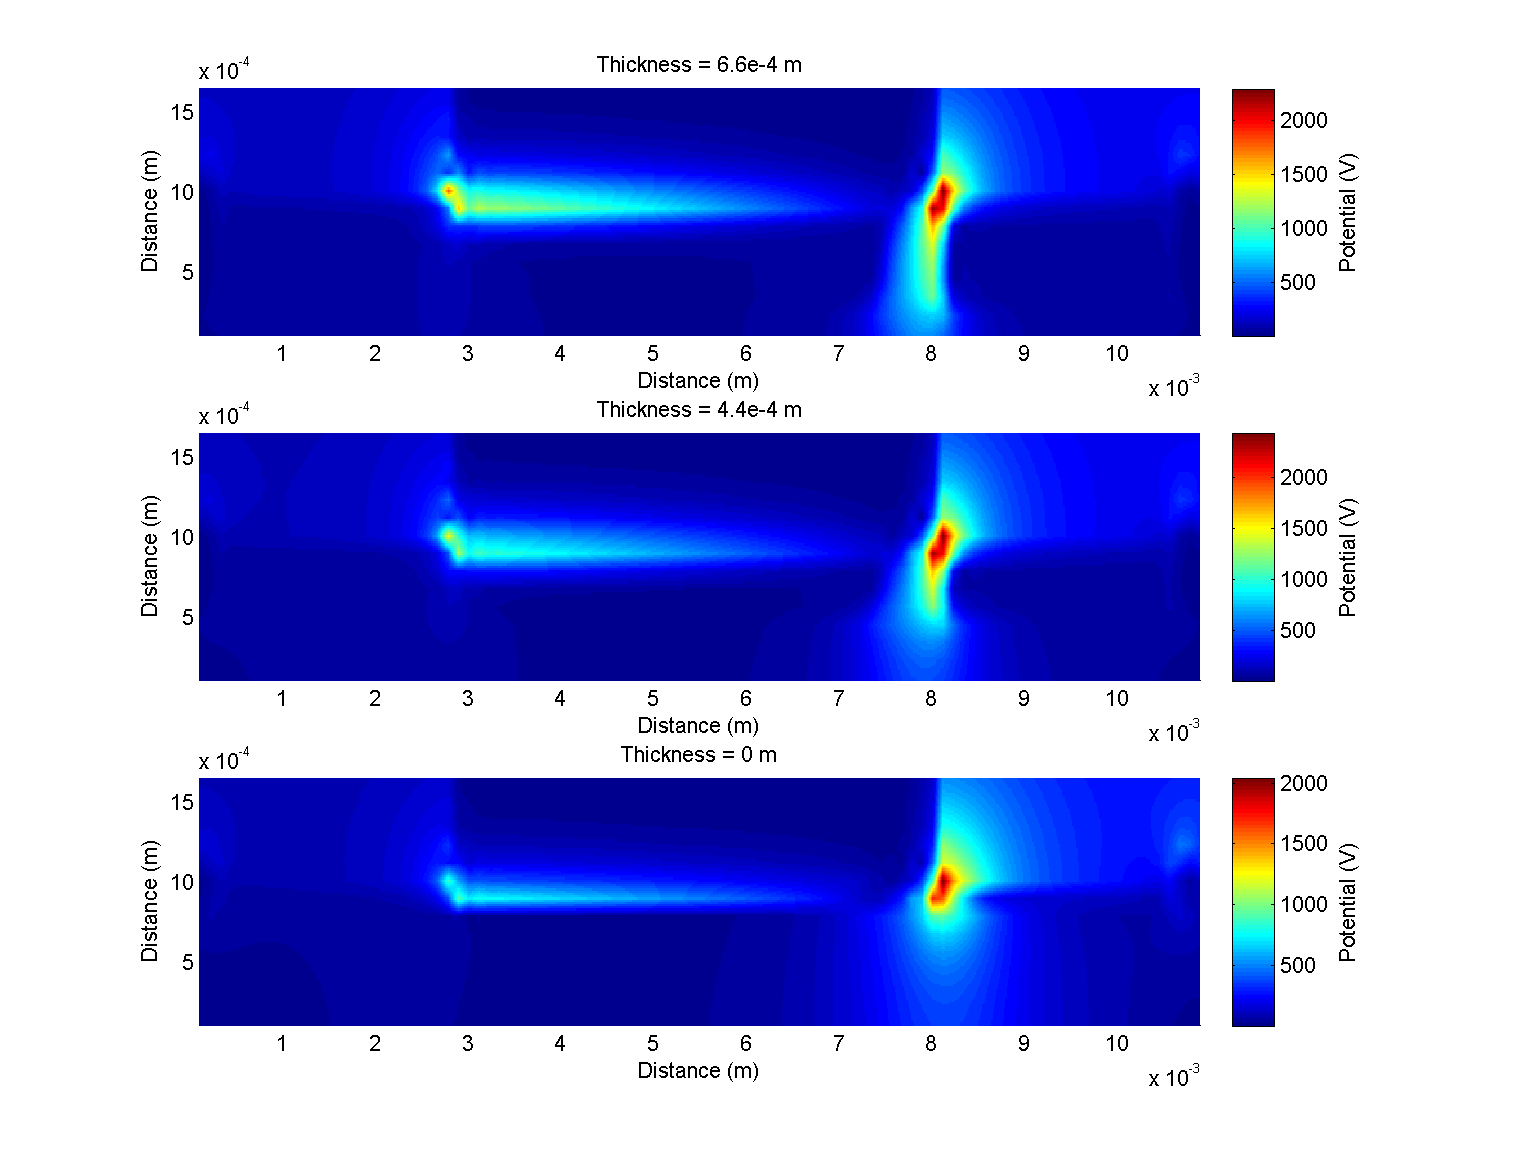
\includegraphics[scale=0.50]{2D_Memristor_Thick_E}
\caption{} 
\label{thick_efield}
\end{figure}


\clearpage
\section{2-D Memristor Simulation Using a Pulse Train}

\begin{figure}[!htp]
\centering
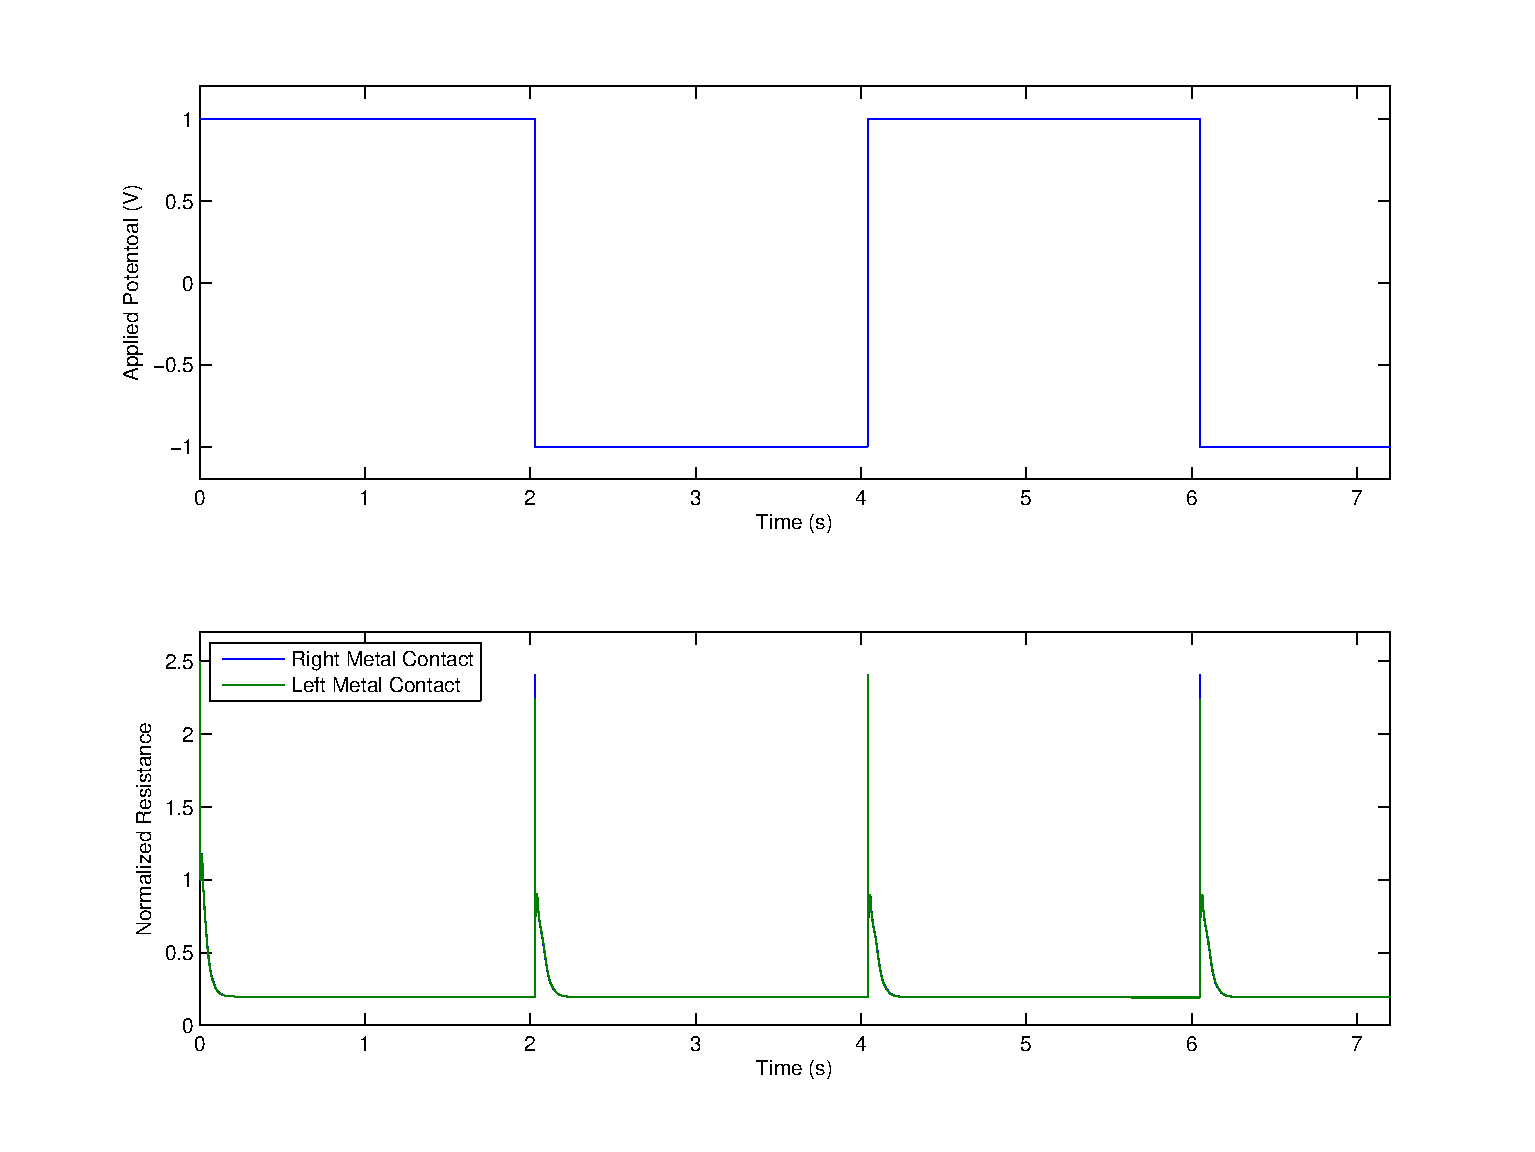
\includegraphics[scale=0.50]{2D_Memristor_Pulse_Train}
\caption{} 
\label{}
\end{figure}


\begin{figure}[!htp]
\centering
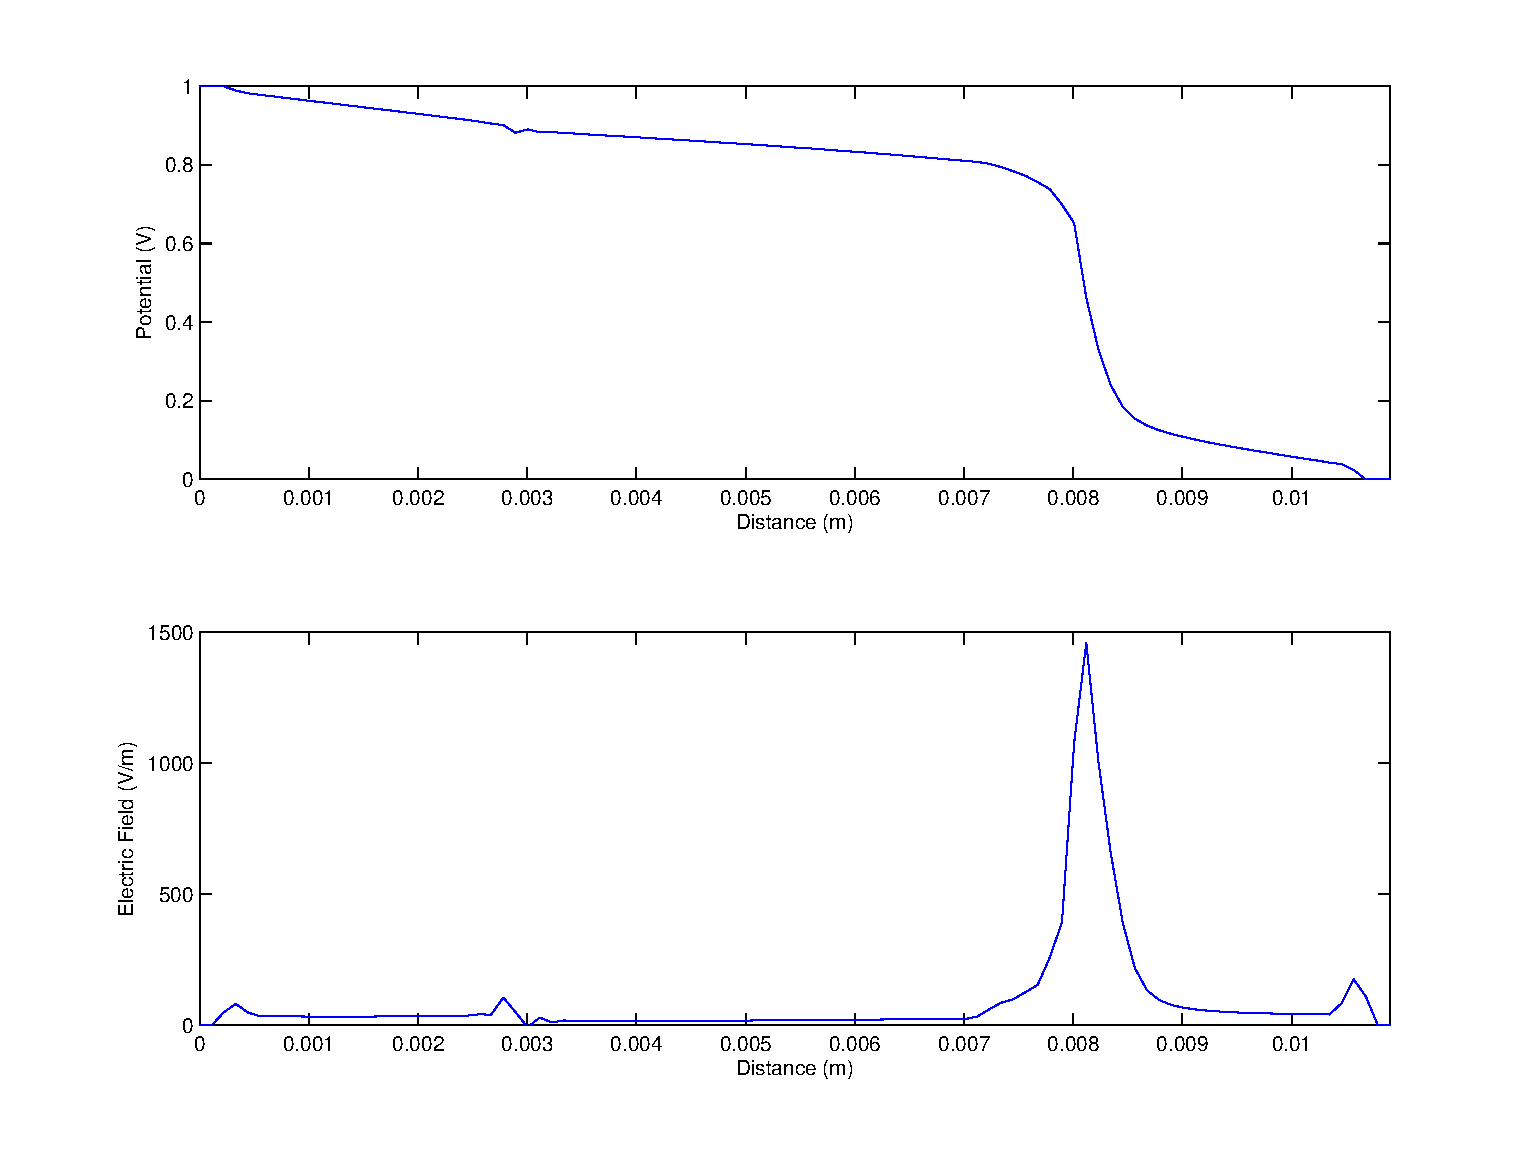
\includegraphics[scale=0.50]{2D_Memristor_Pulse_Train_EV}
\caption{} 
\label{}
\end{figure}

\begin{figure}[!htp]
\centering
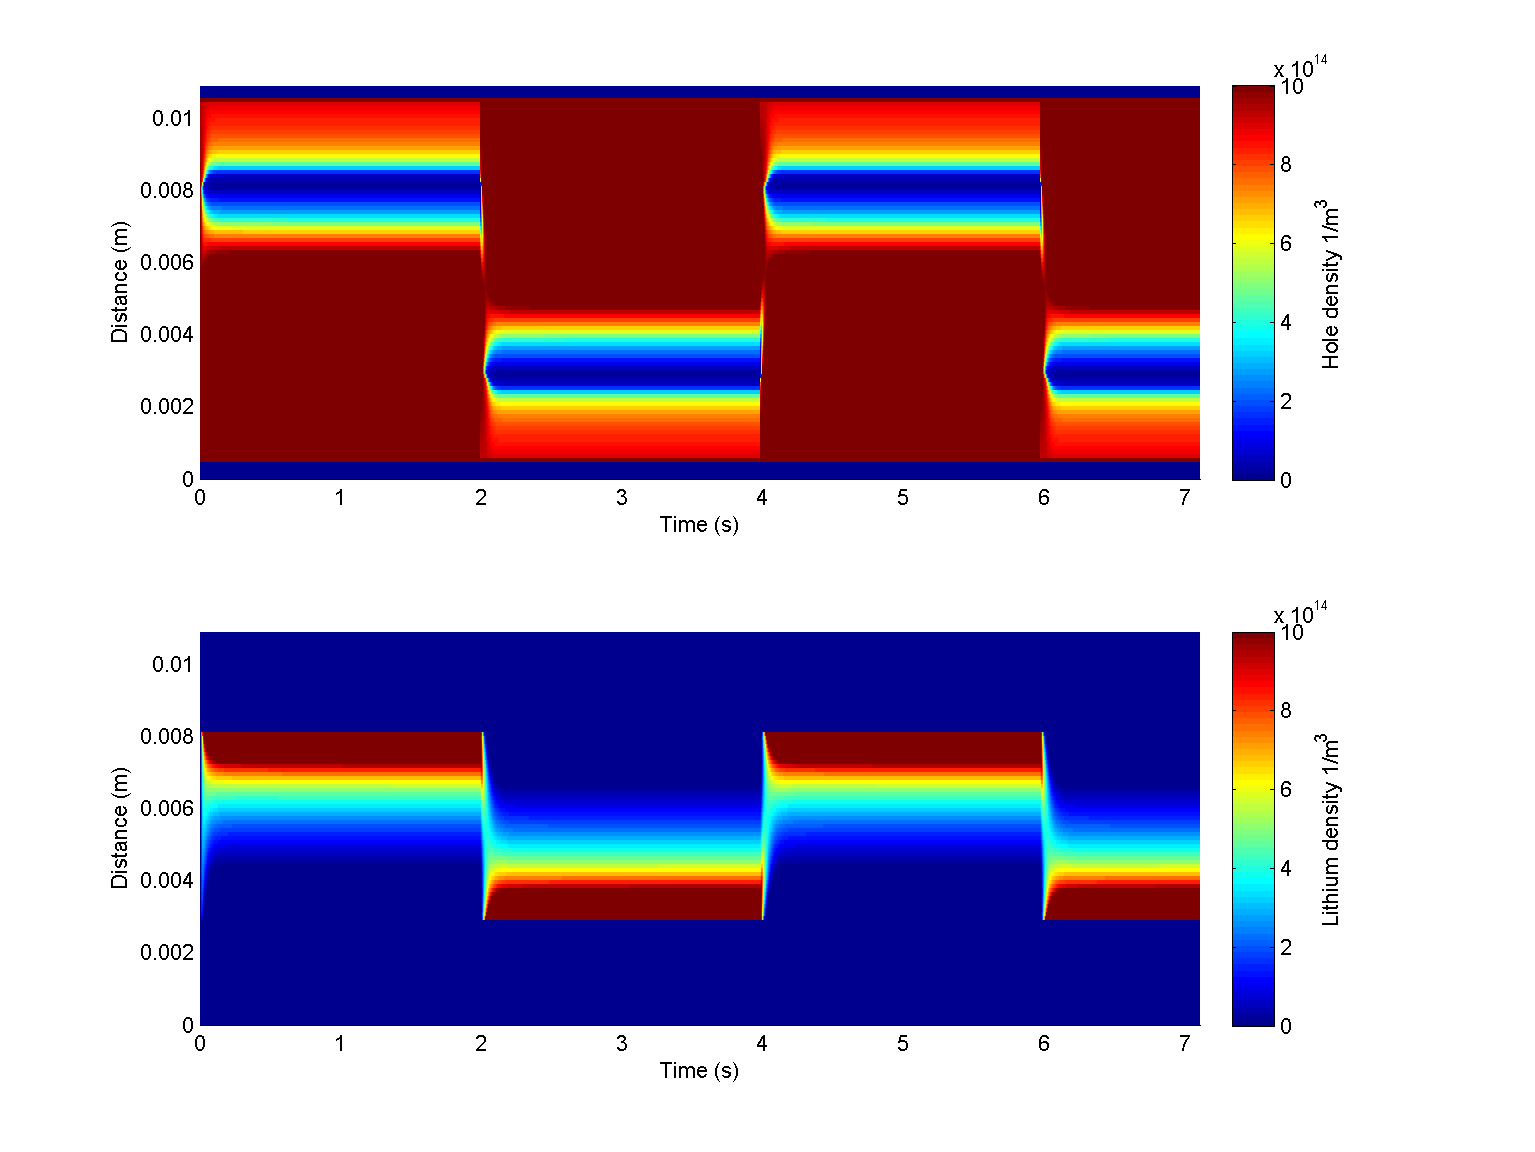
\includegraphics[scale=0.50]{2D_Memristor_Pulse_Lithium_Hole}
\caption{} 
\label{}
\end{figure}

\begin{figure}[!htp]
\centering
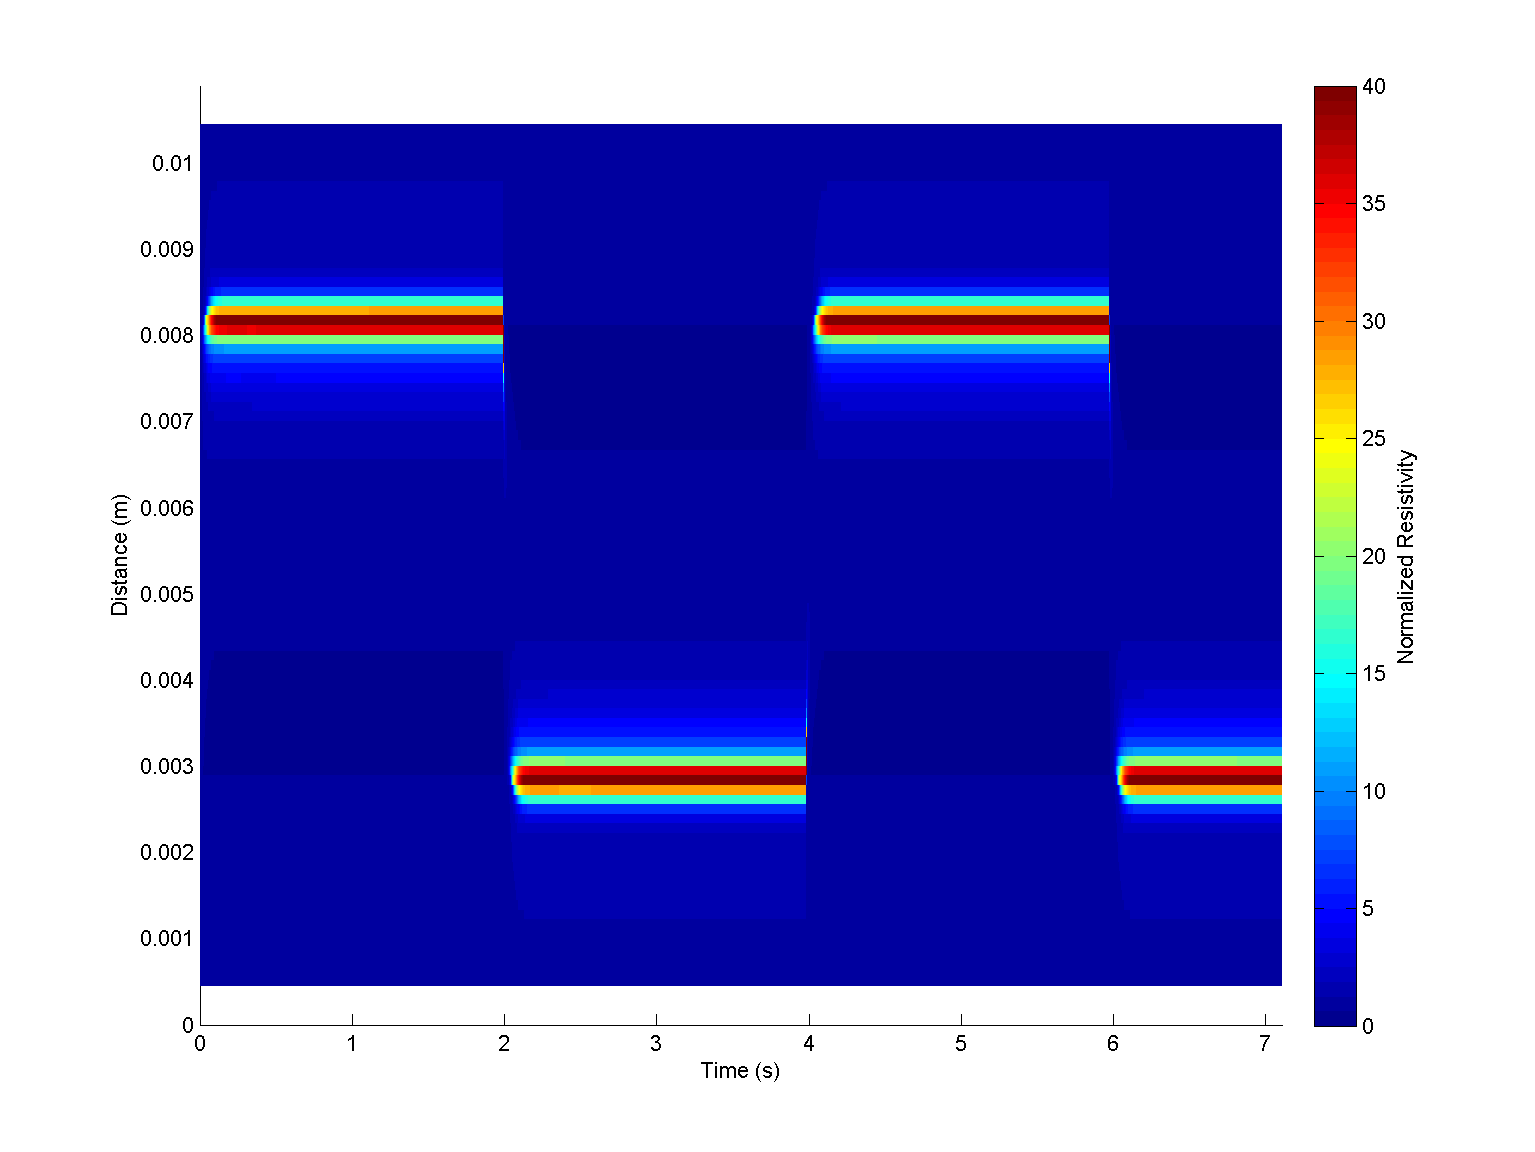
\includegraphics[scale=0.50]{2D_Memristor_Resistivity}
\caption{} 
\label{}
\end{figure}



\begin{figure}[!htp]
\centering
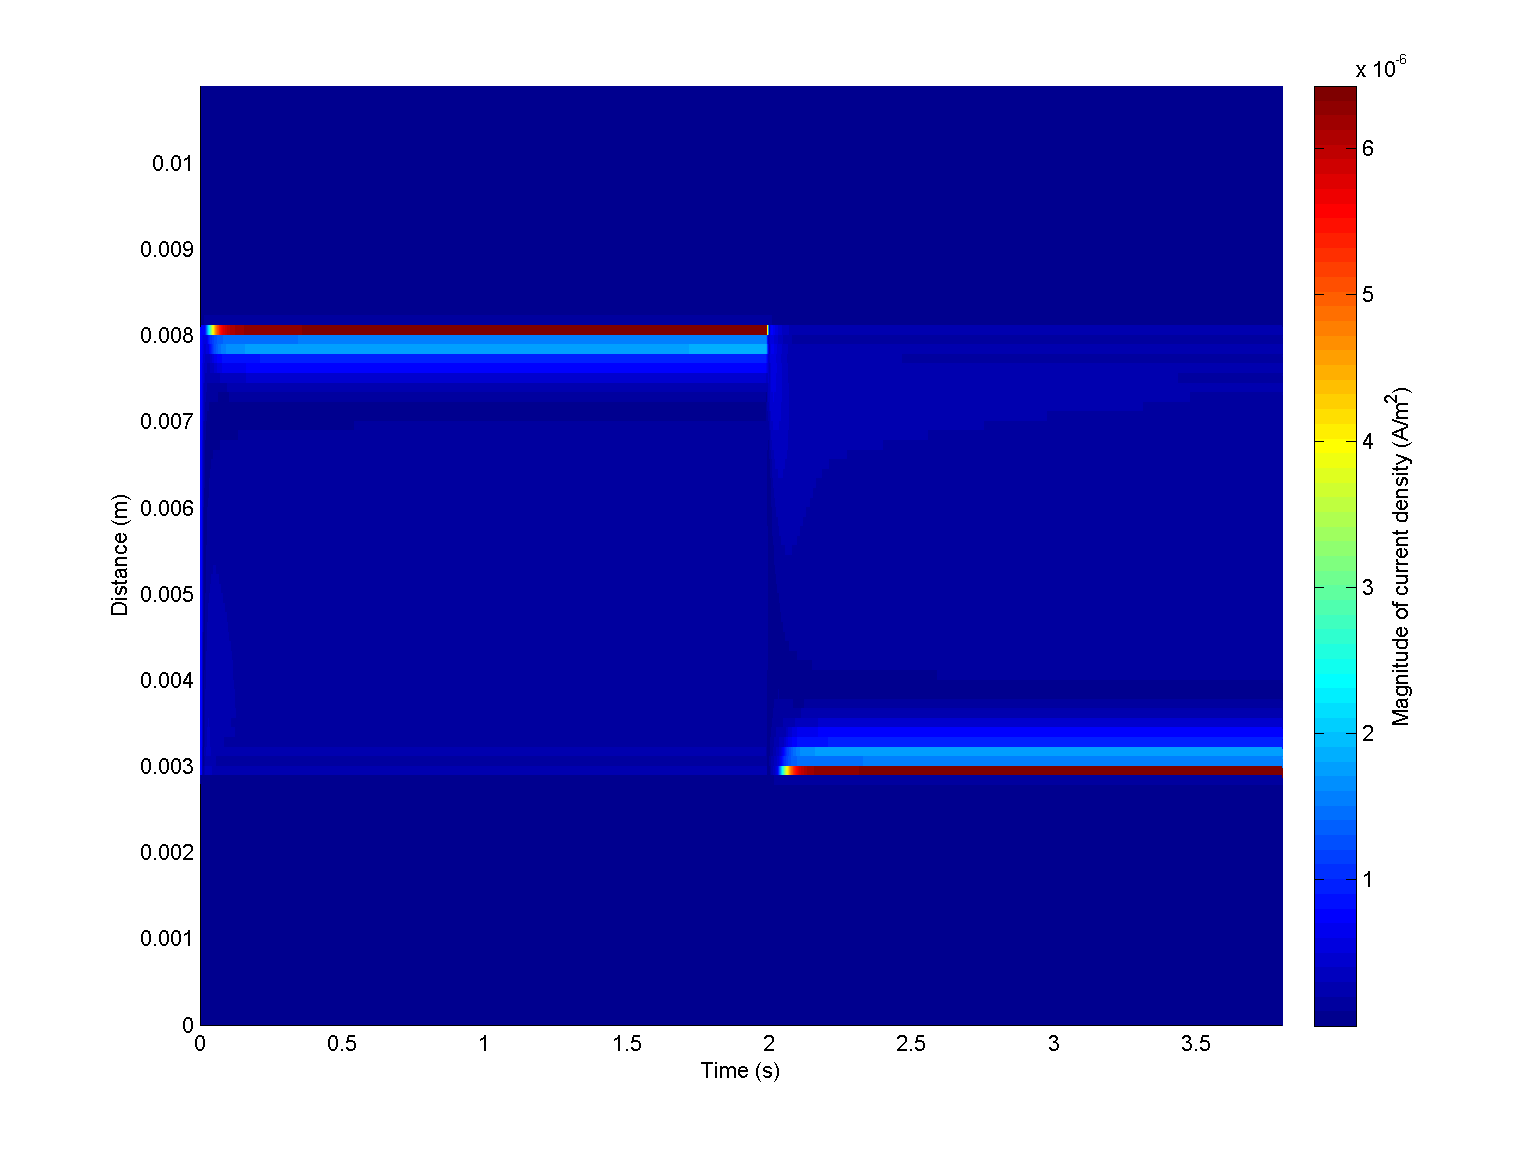
\includegraphics[scale=0.50]{2D_Memristor_Pulse_Lithium_J}
\caption{} 
\label{}
\end{figure}


\clearpage
\section{2-D Memristor Simulation Using a Sinusoid}

\begin{figure}[!htp]
\centering
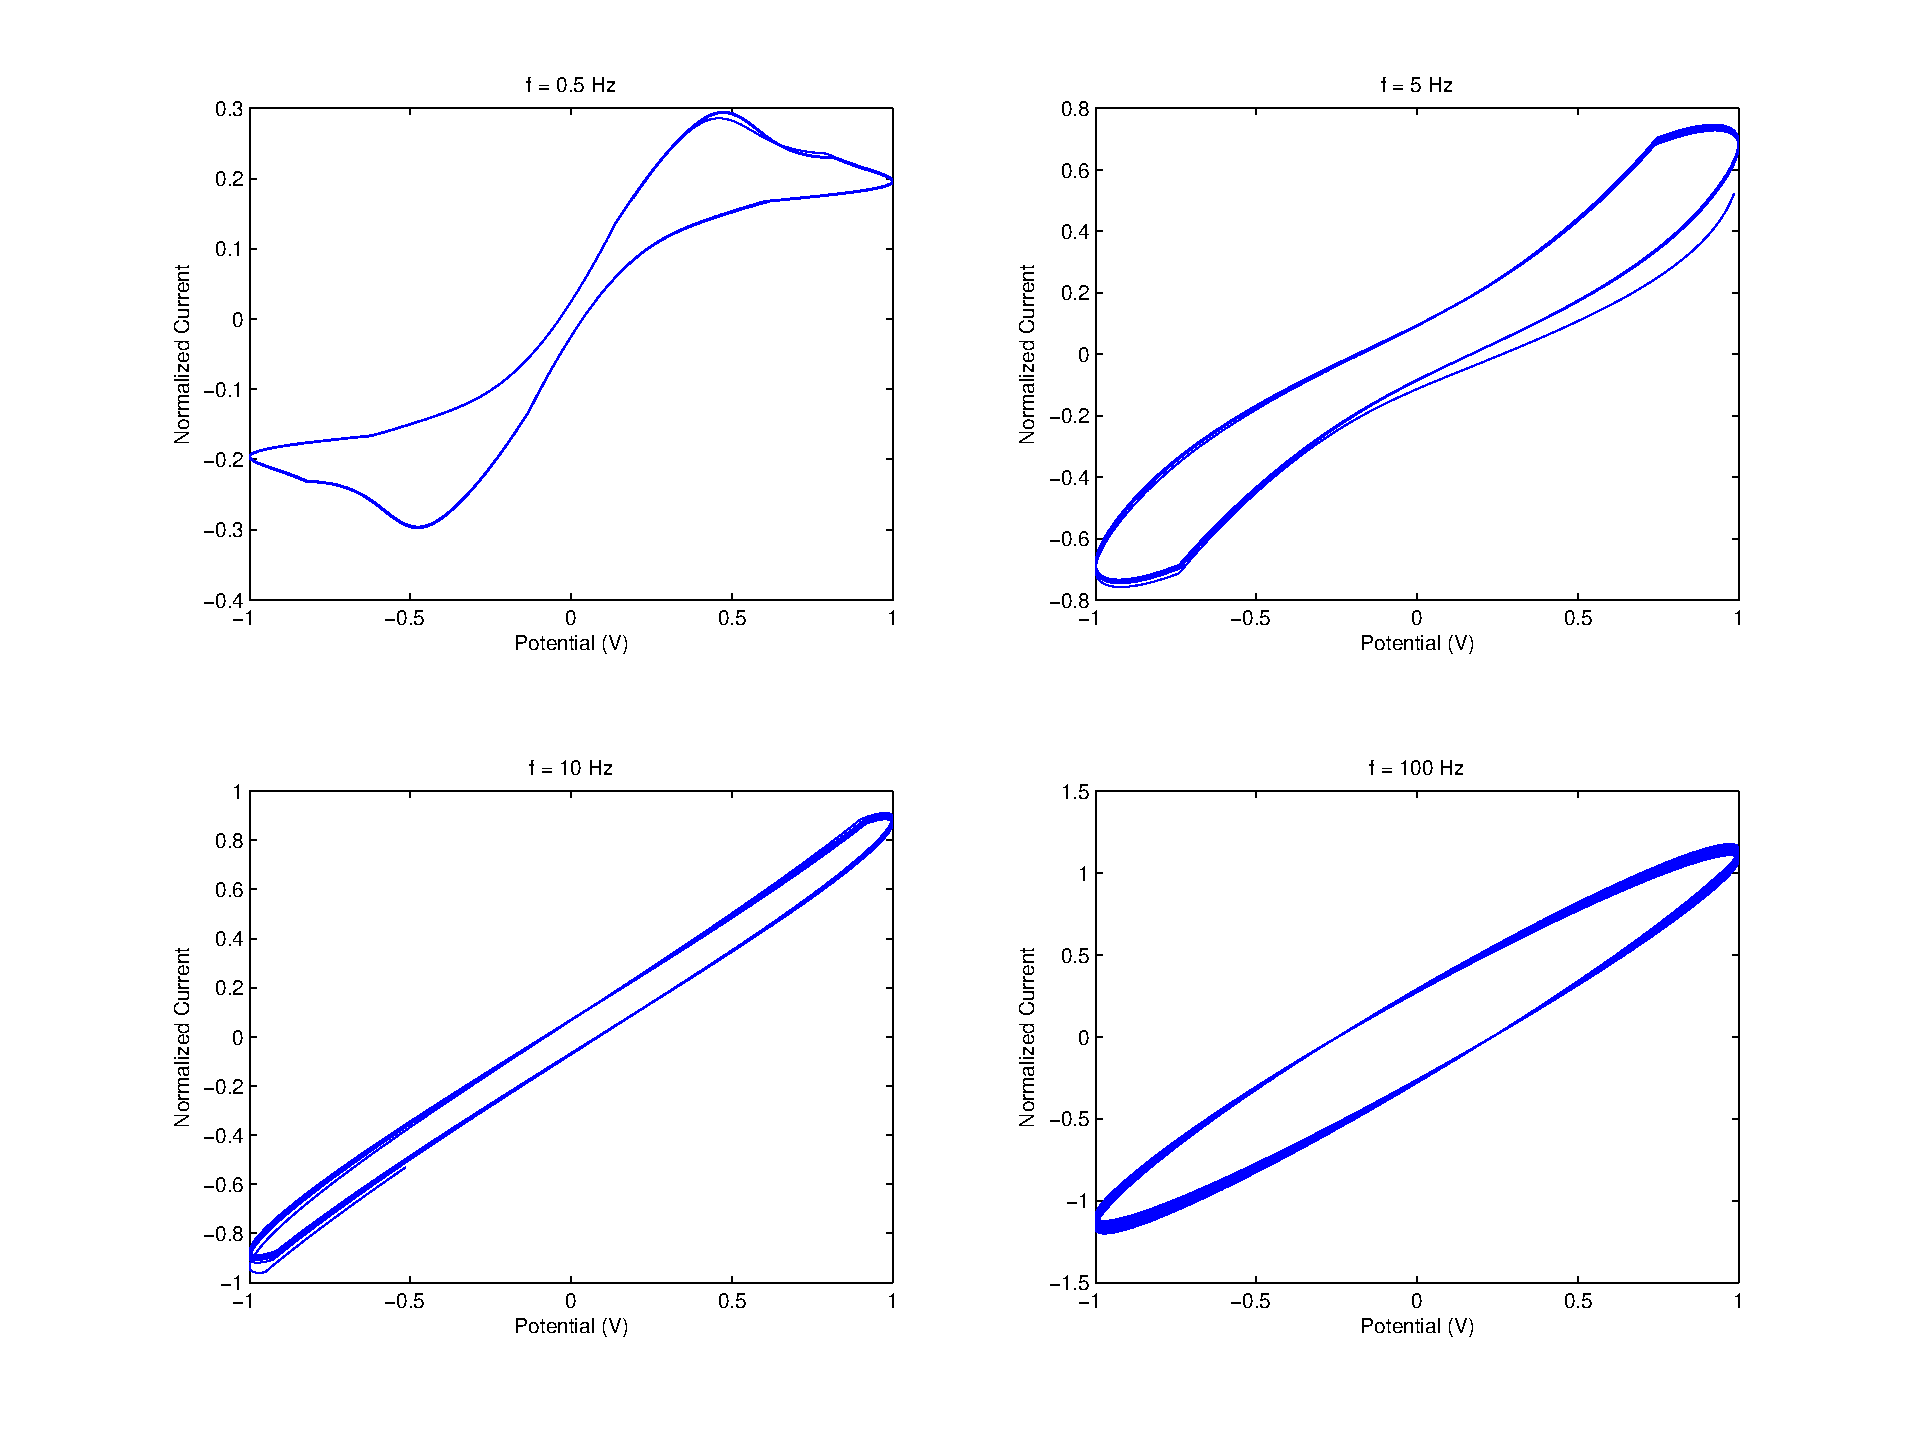
\includegraphics[scale=0.45]{2D_Memristor_bowtie_f}
\caption{} 
\label{}
\end{figure}


\begin{figure}[!htp]
\centering
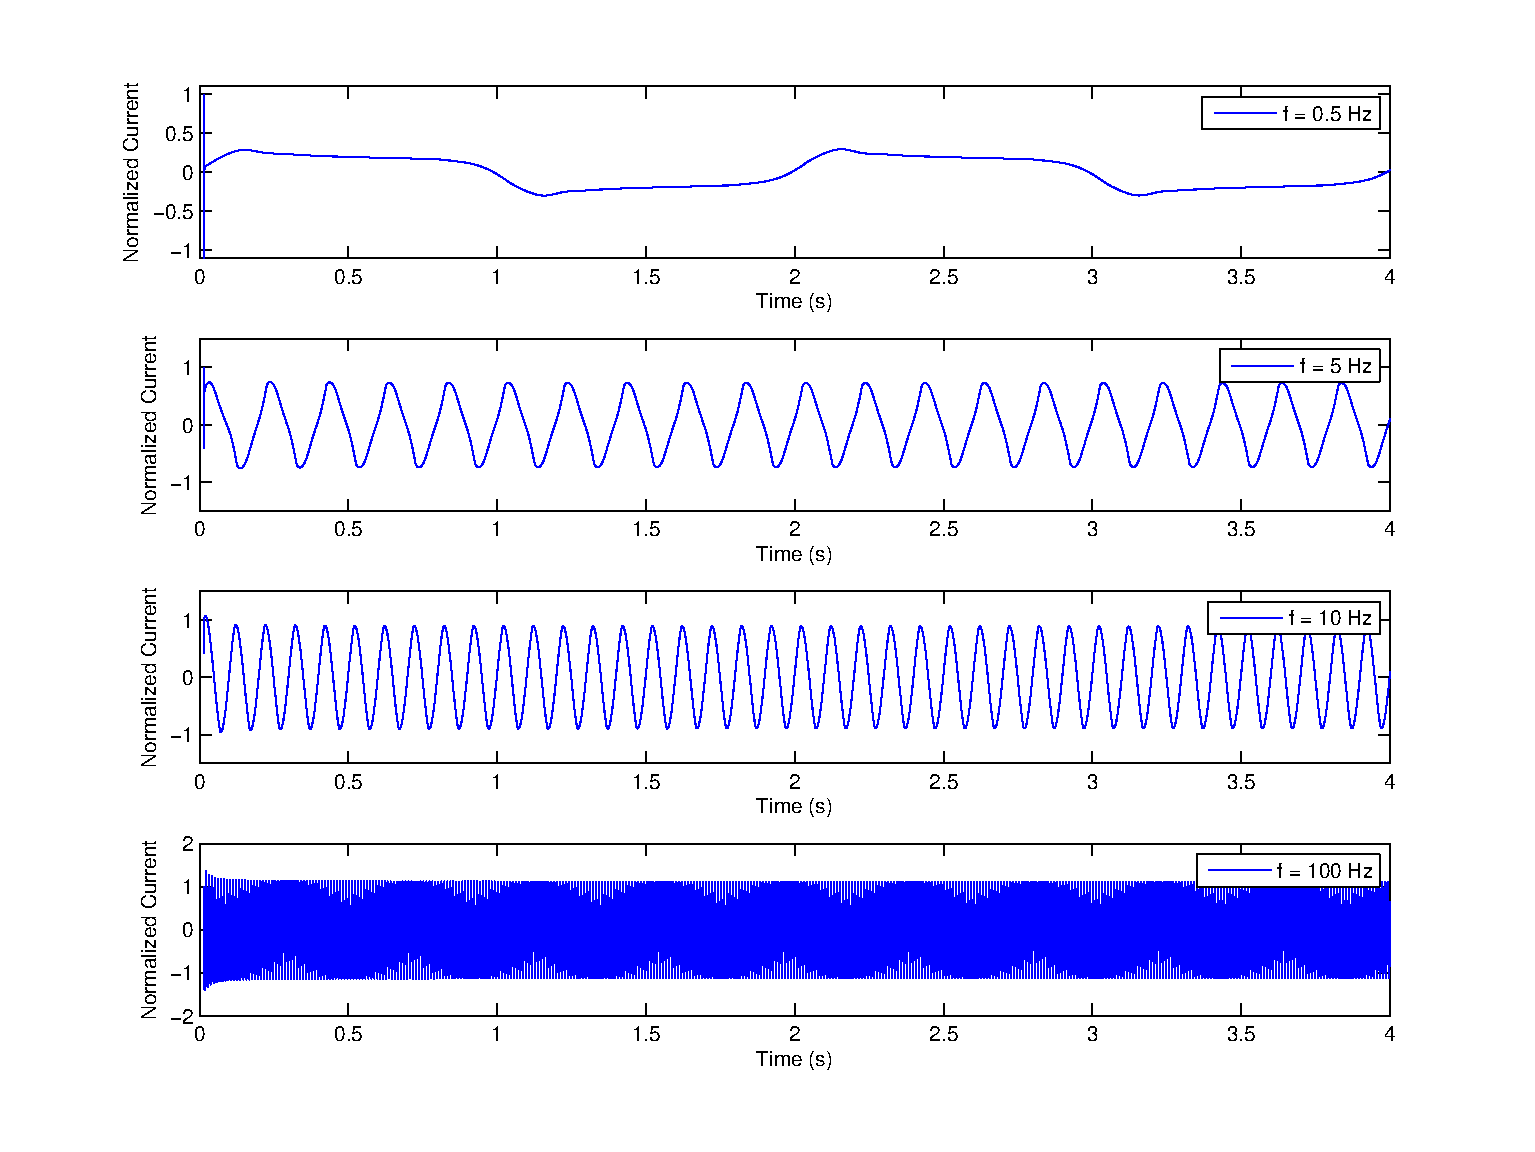
\includegraphics[scale=0.50]{2D_Memristor_Current_f}
\caption{} 
\label{}
\end{figure}

\begin{figure}[!htp]
\centering
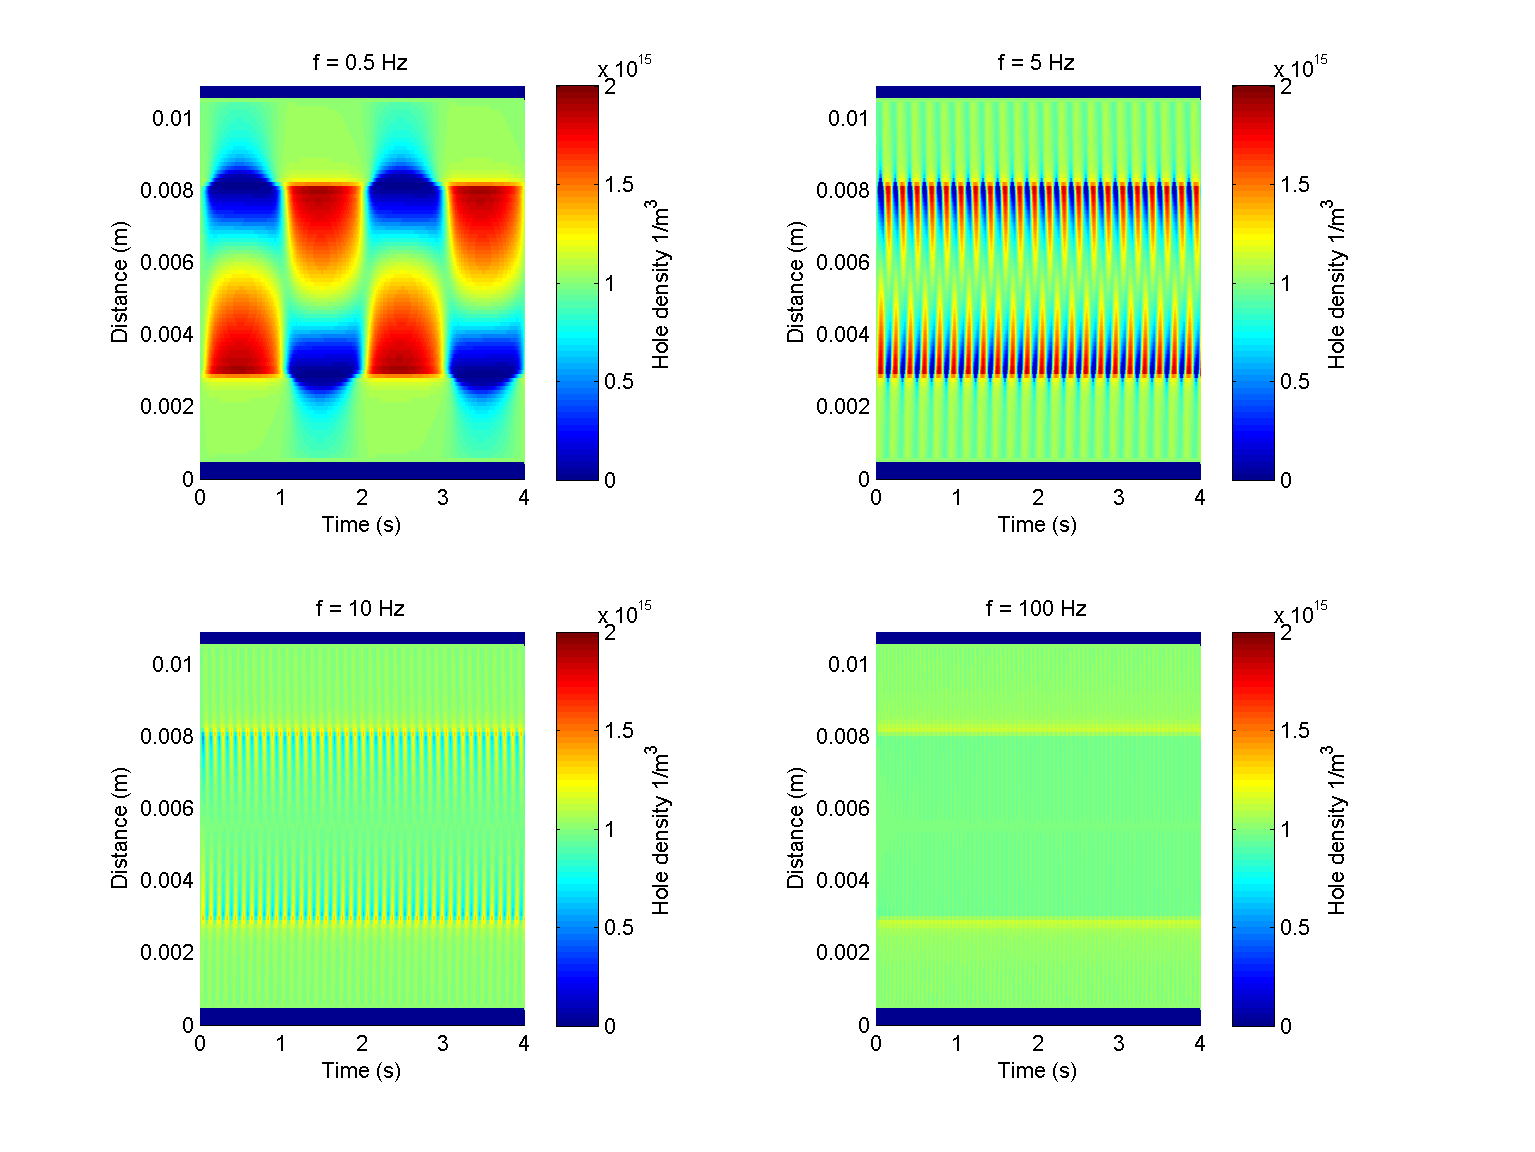
\includegraphics[scale=0.55]{2D_Memristor_f_Hole}
\caption{} 
\label{}
\end{figure}

\begin{figure}[!htp]
\centering
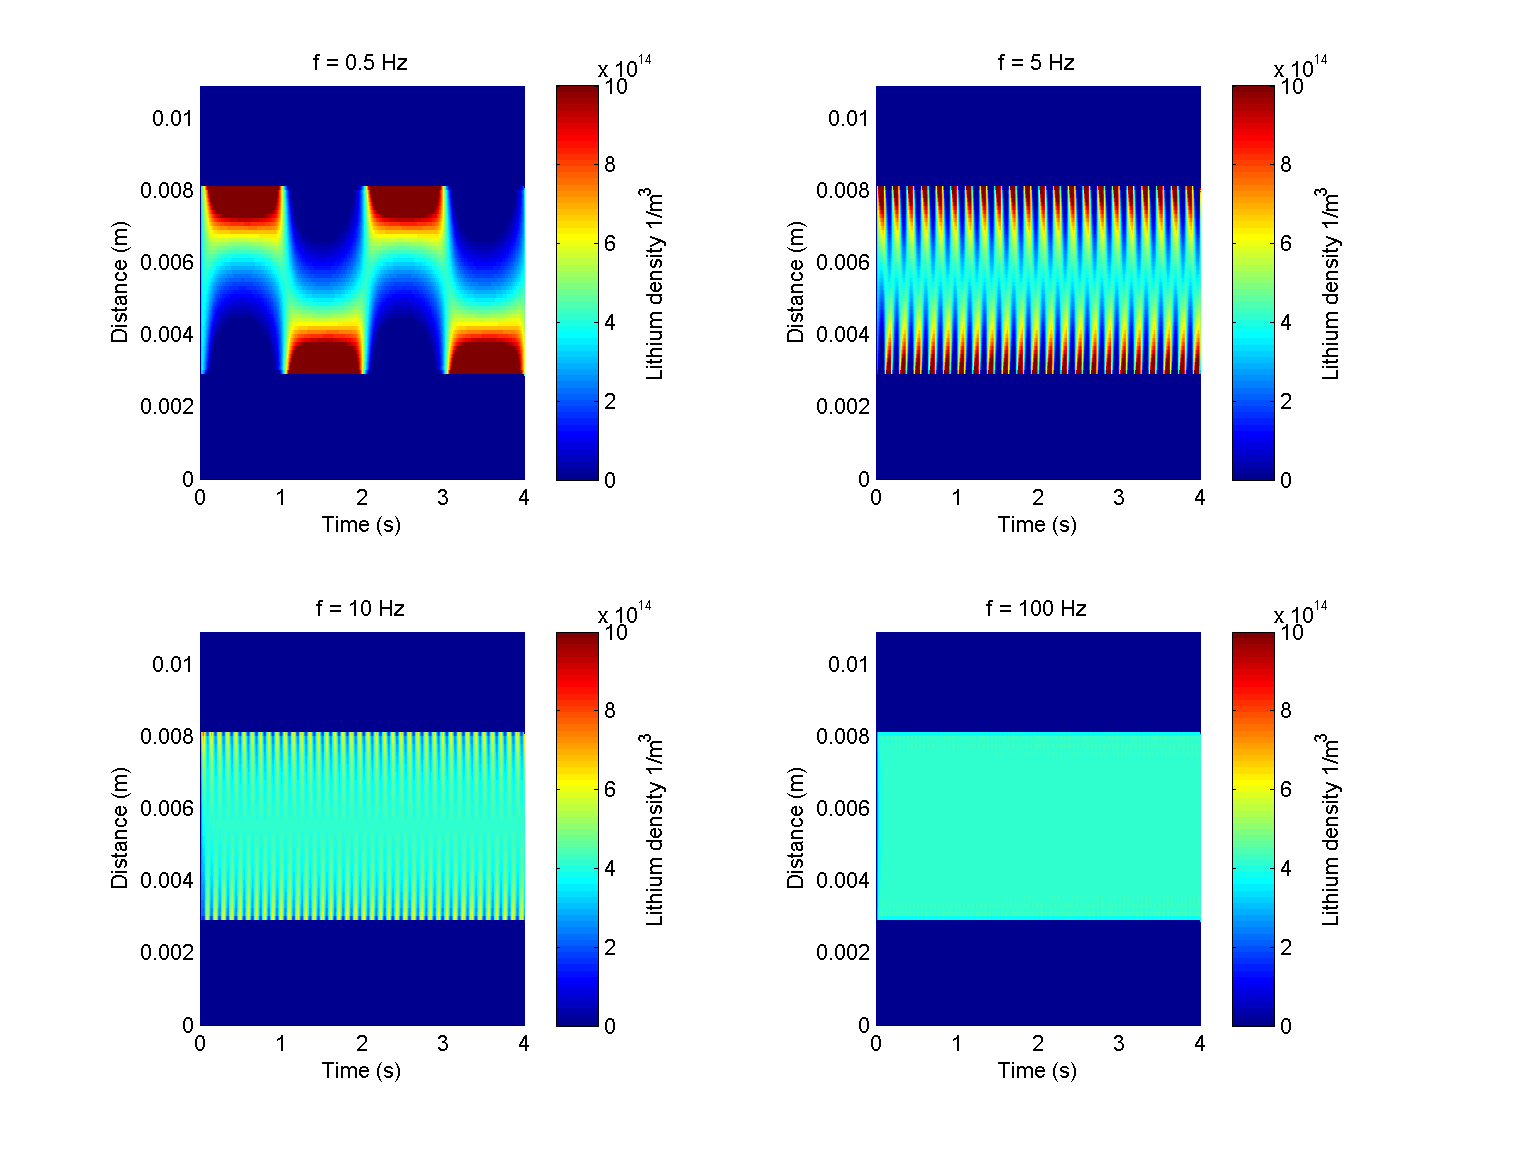
\includegraphics[scale=0.55]{2D_Memristor_f_Lithium}
\caption{} 
\label{}
\end{figure}

\begin{figure}[!htp]
\centering
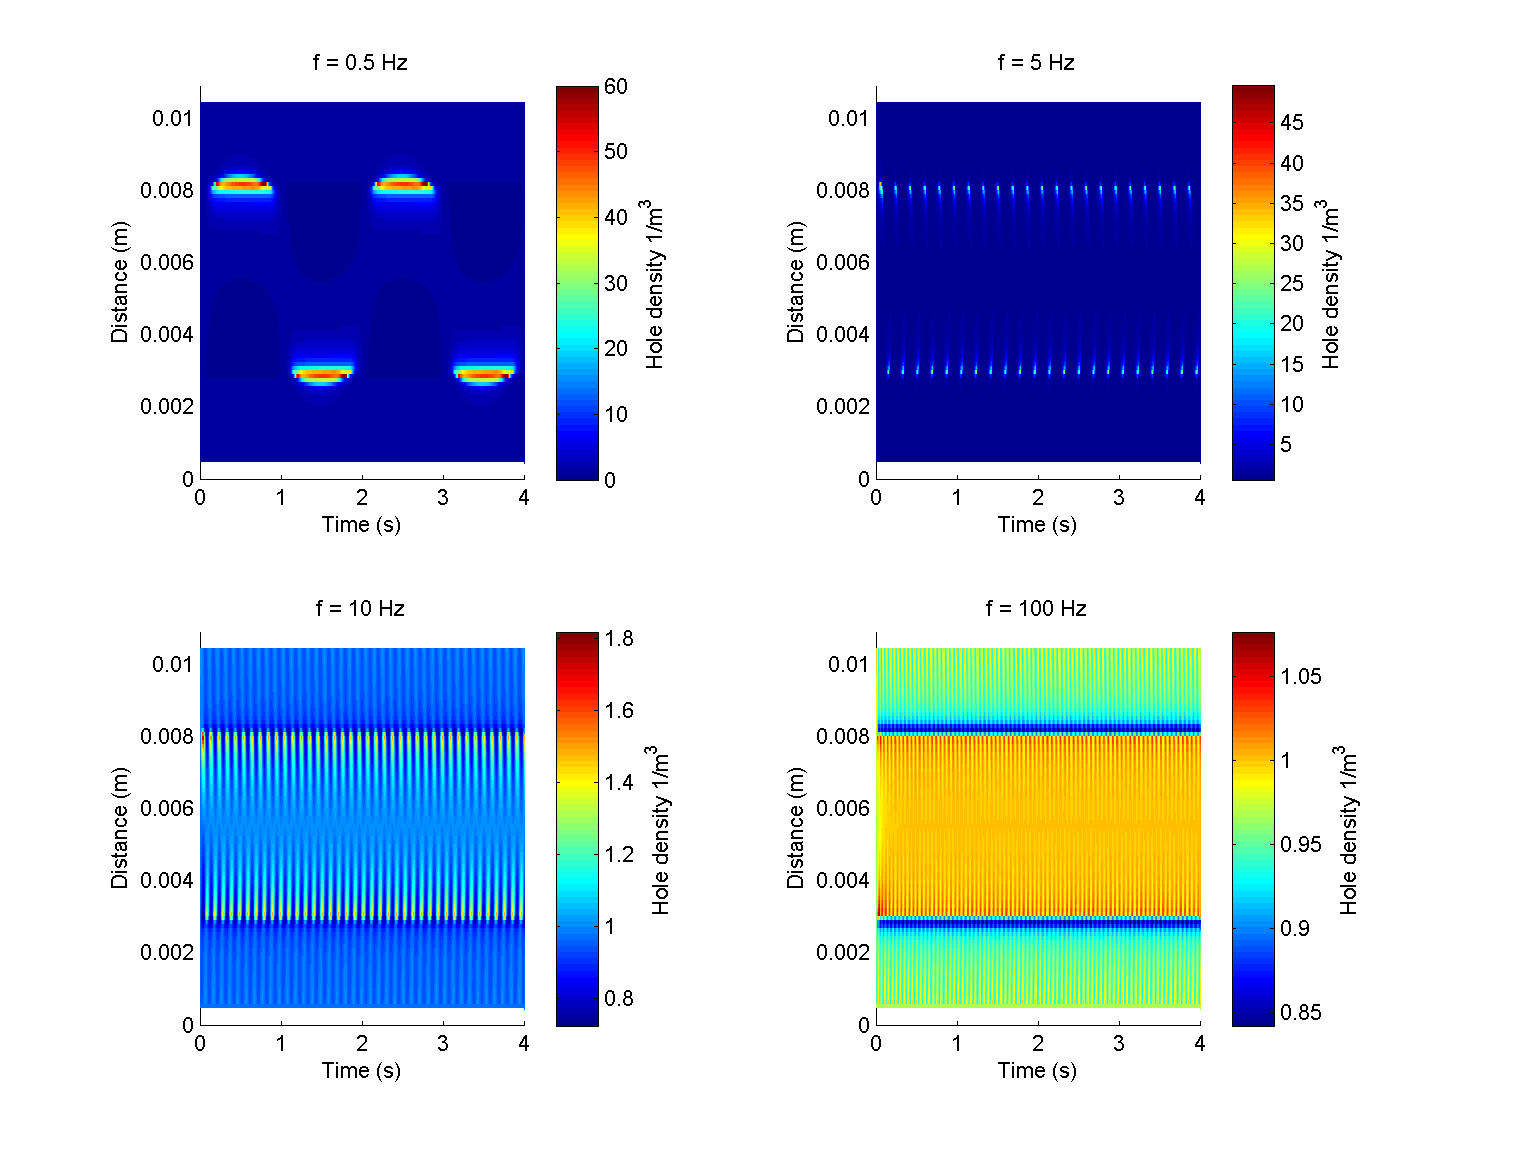
\includegraphics[scale=0.55]{2D_Memristor_f_Resistivity}
\caption{} 
\label{}
\end{figure}


\begin{figure}[!htp]
\centering
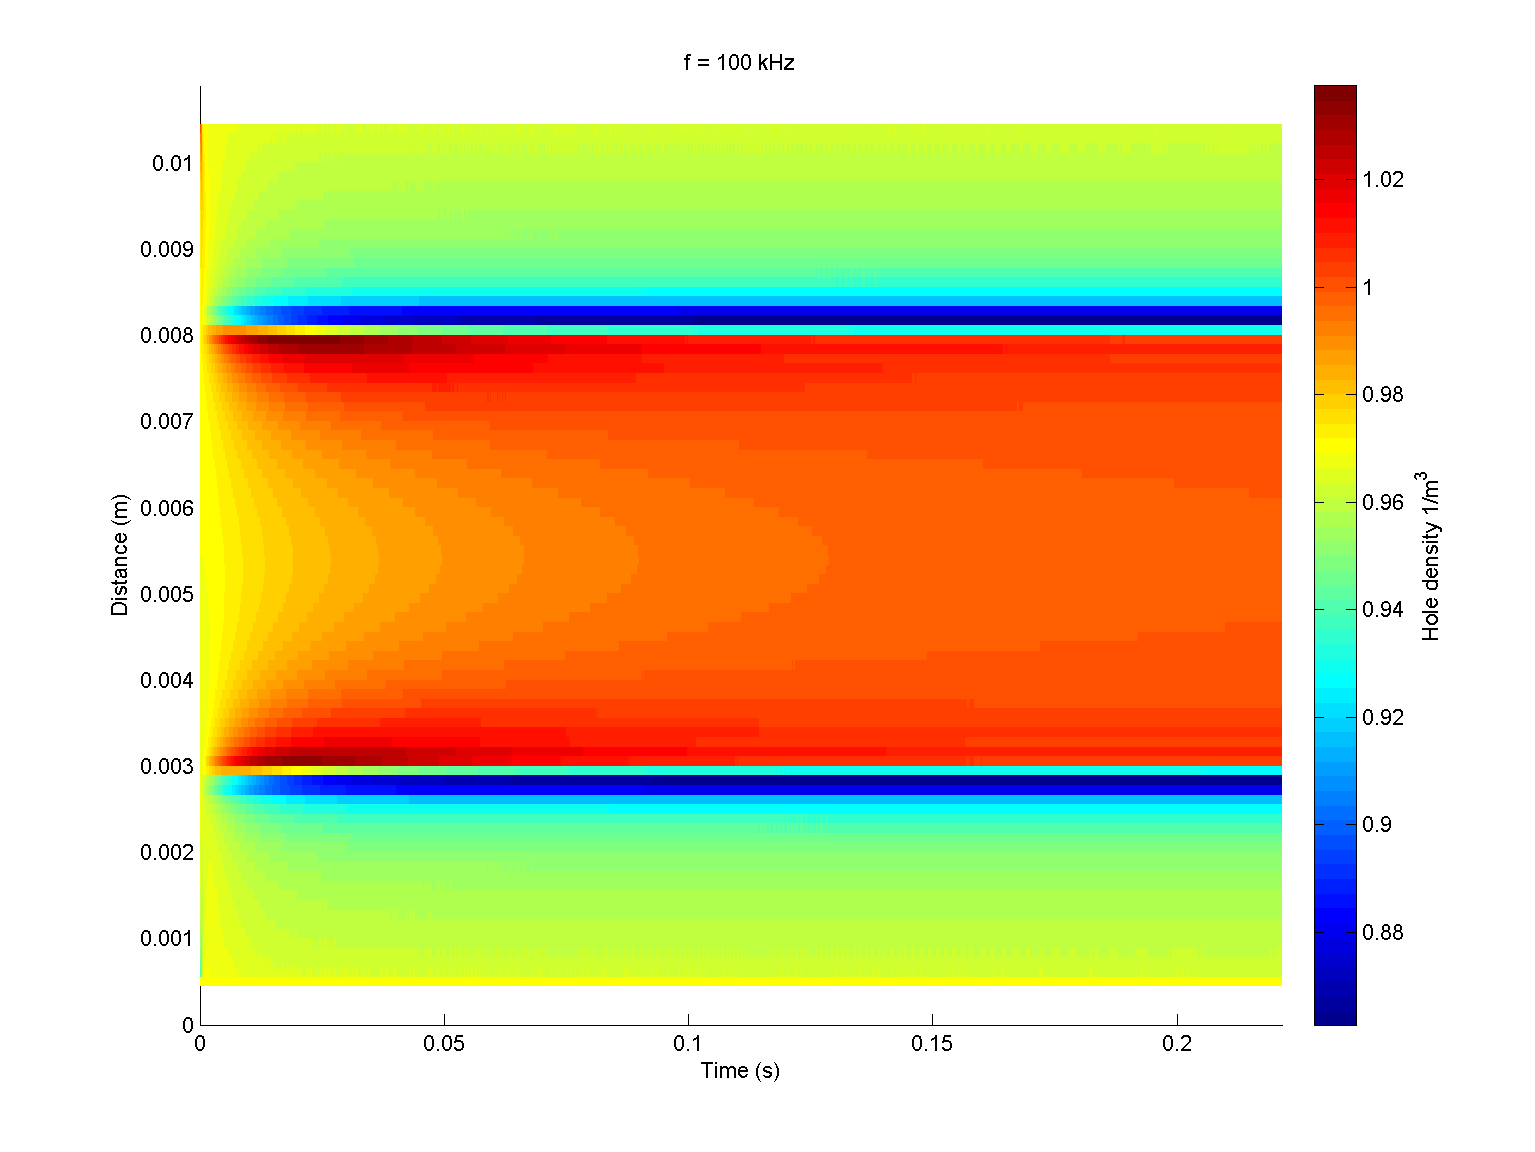
\includegraphics[scale=0.50]{2D_Memristor_f_Resistivity_1e5}
\caption{} 
\label{}
\end{figure}

\clearpage
\section{Experiment vs. Simulation}


\begin{figure}[!htp]
\centering
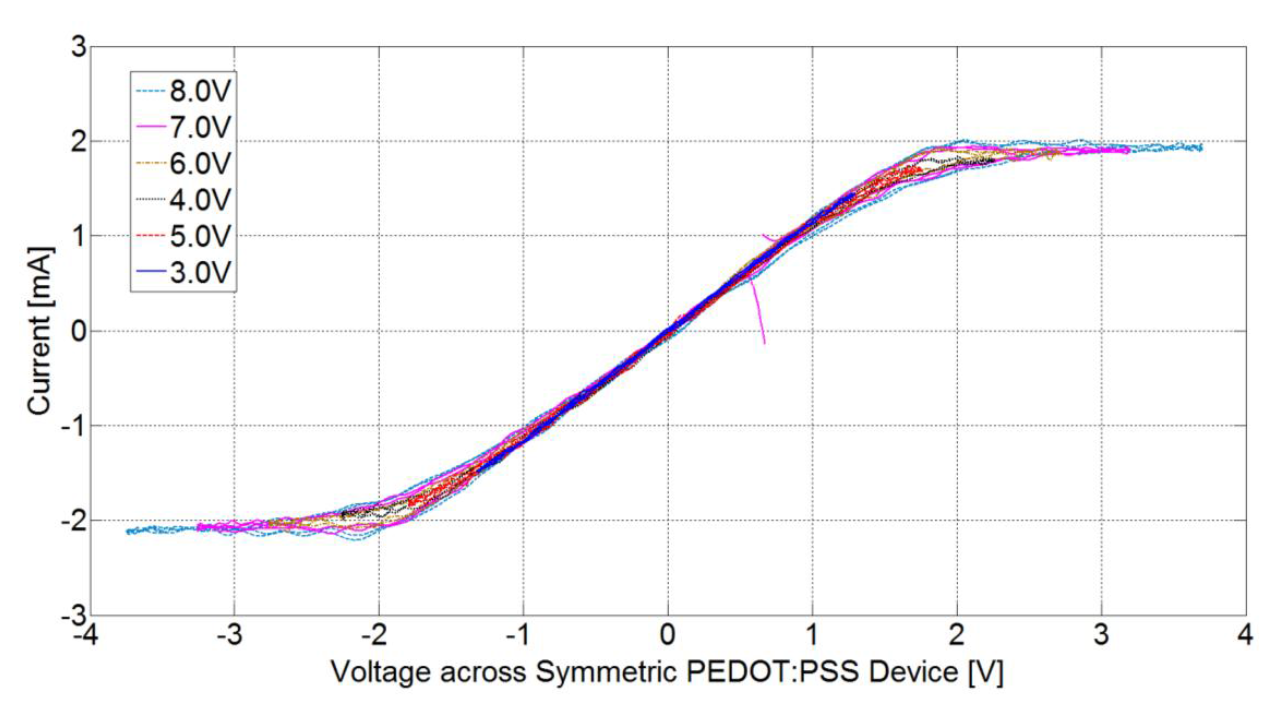
\includegraphics[scale=0.33]{memf1e-1}
\caption{} 
\label{}
\end{figure}


\begin{figure}[!htp]
\centering
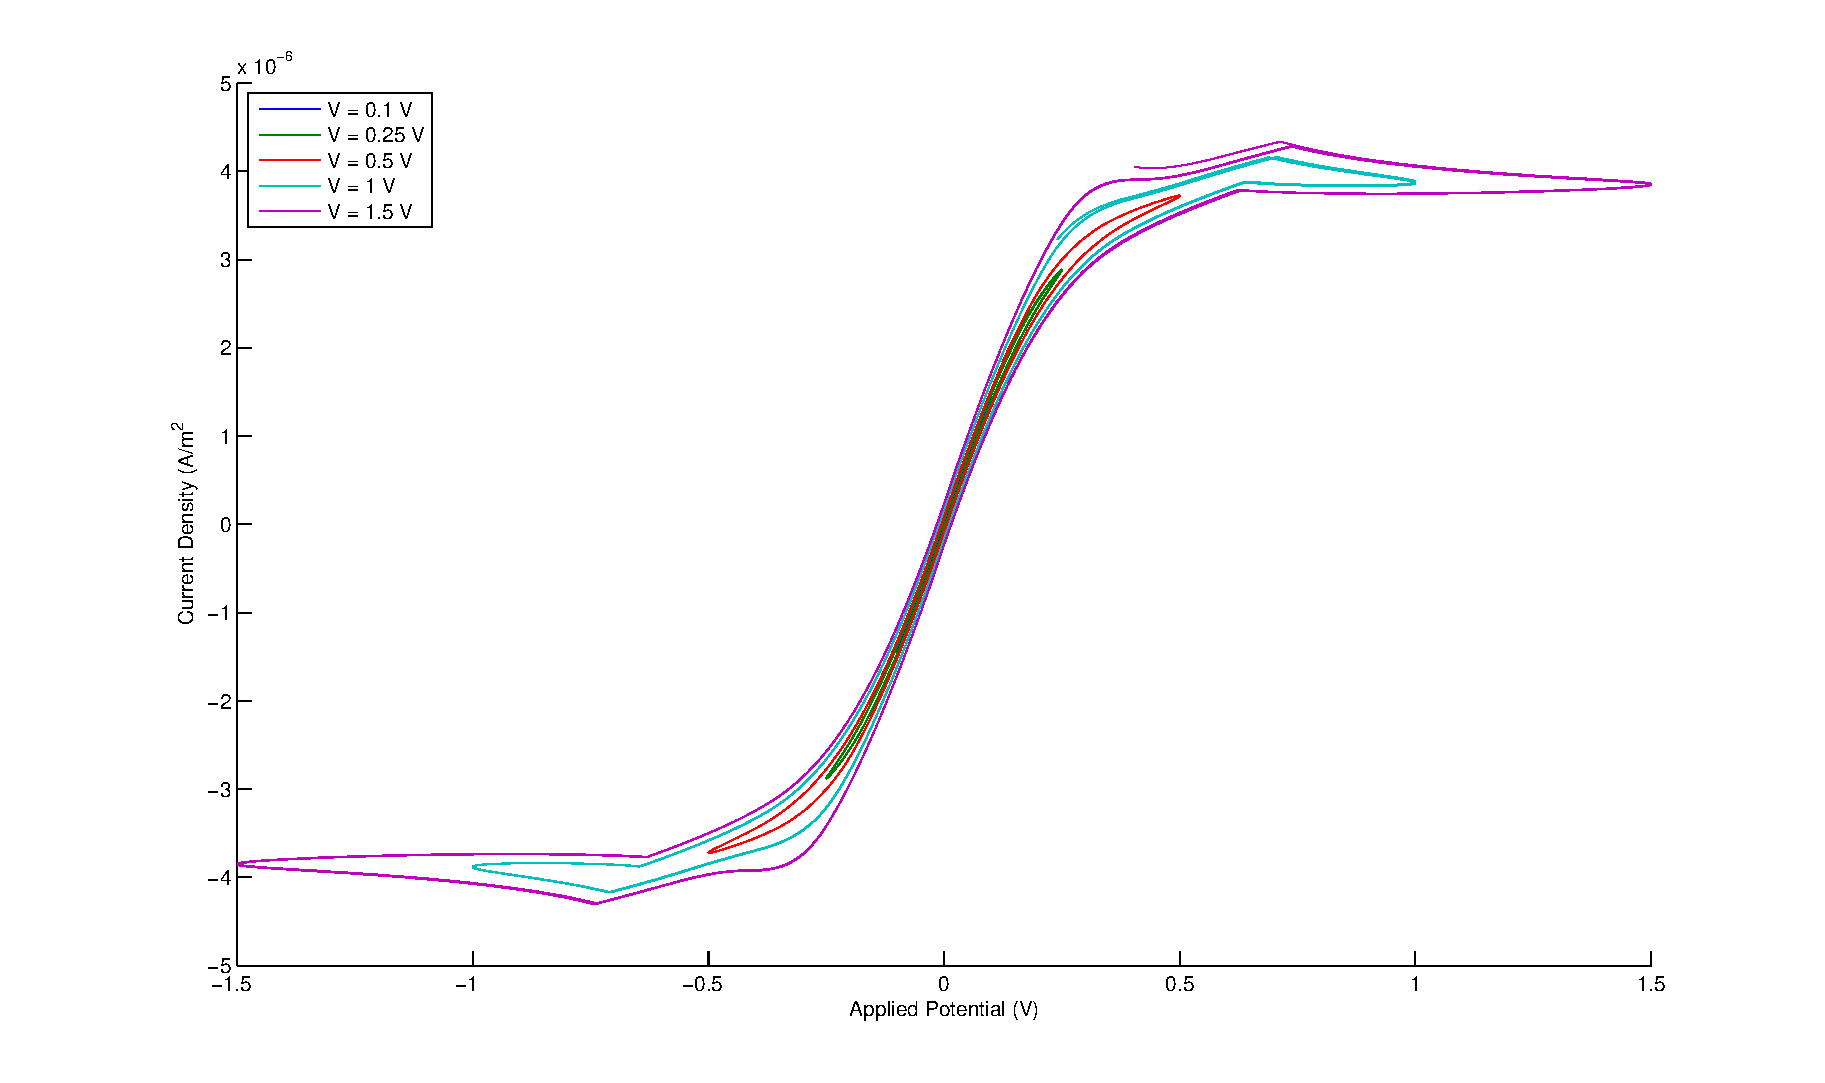
\includegraphics[scale=0.36]{Bowtief01Vchng}
\caption{} 
\label{}
\end{figure}


\begin{figure}[!htp]
\centering
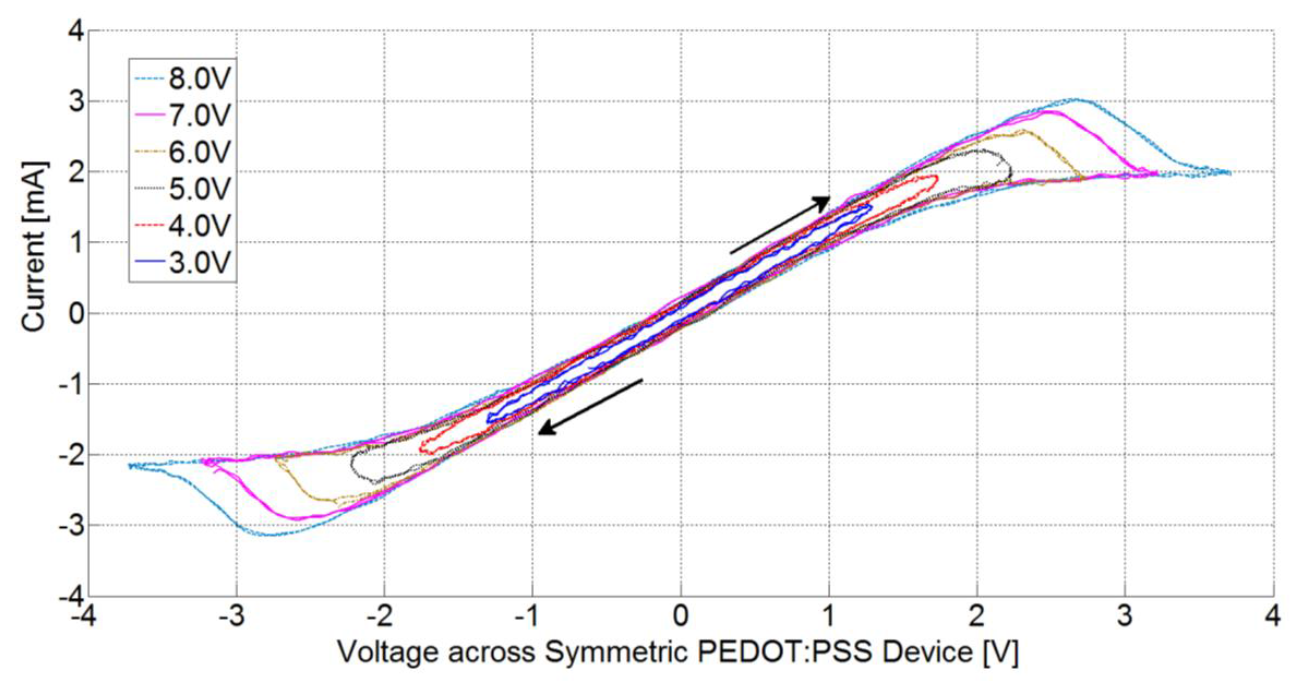
\includegraphics[scale=0.3]{memf1}
\caption{} 
\label{}
\end{figure}


\begin{figure}[!htp]
\centering
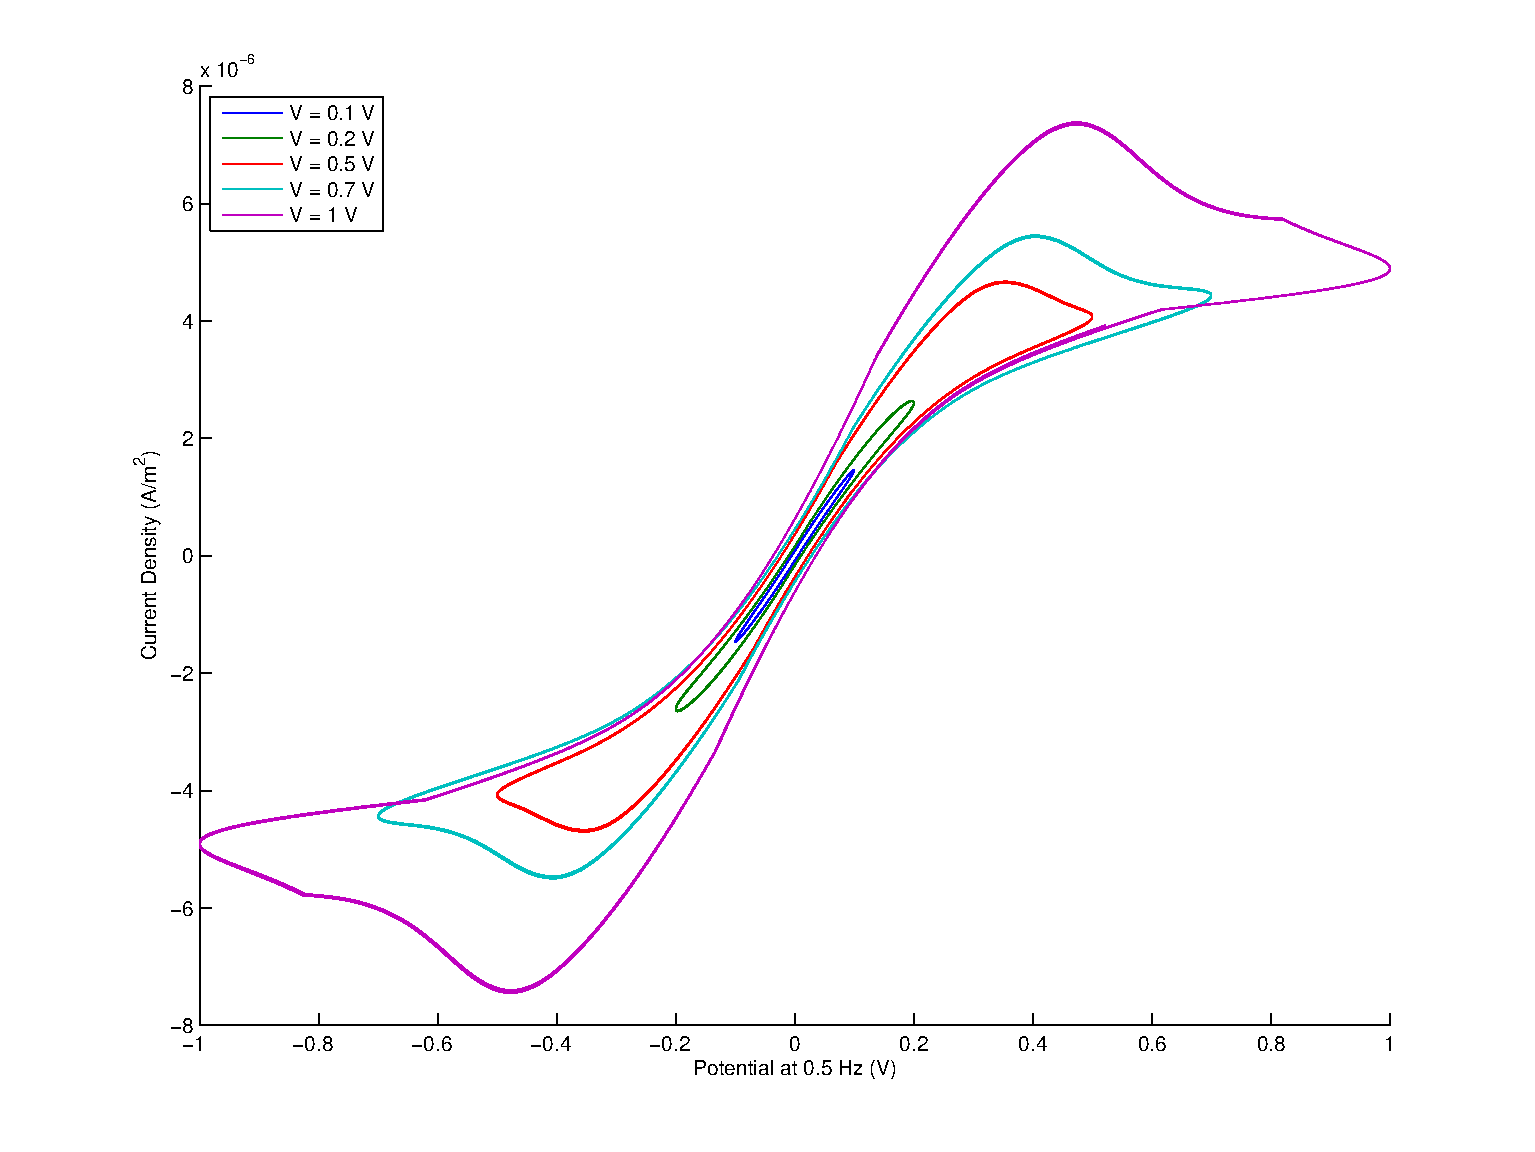
\includegraphics[scale=0.45]{2D_Memristor_5e-1Hz}
\caption{} 
\label{}
\end{figure}


\begin{figure}[!htp]
\centering
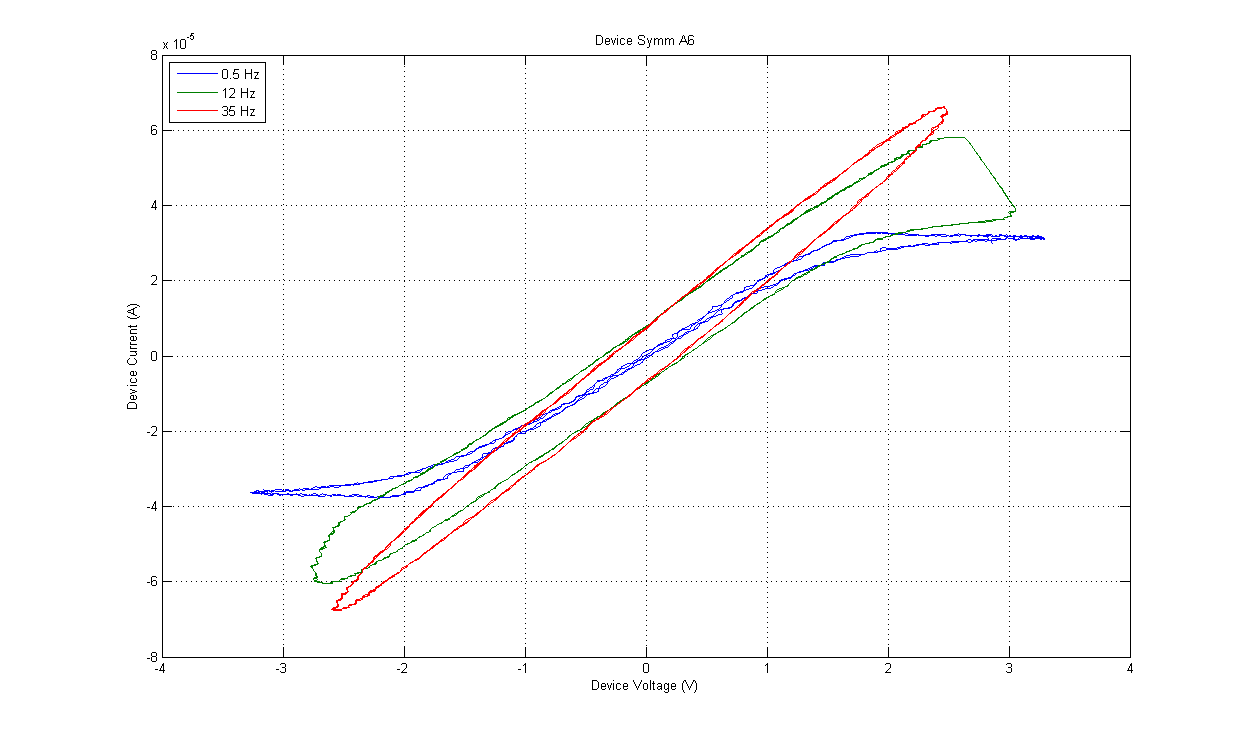
\includegraphics[scale=0.35]{experimental}
\caption{} 
\label{}
\end{figure}

\begin{figure}[!htp]
\centering
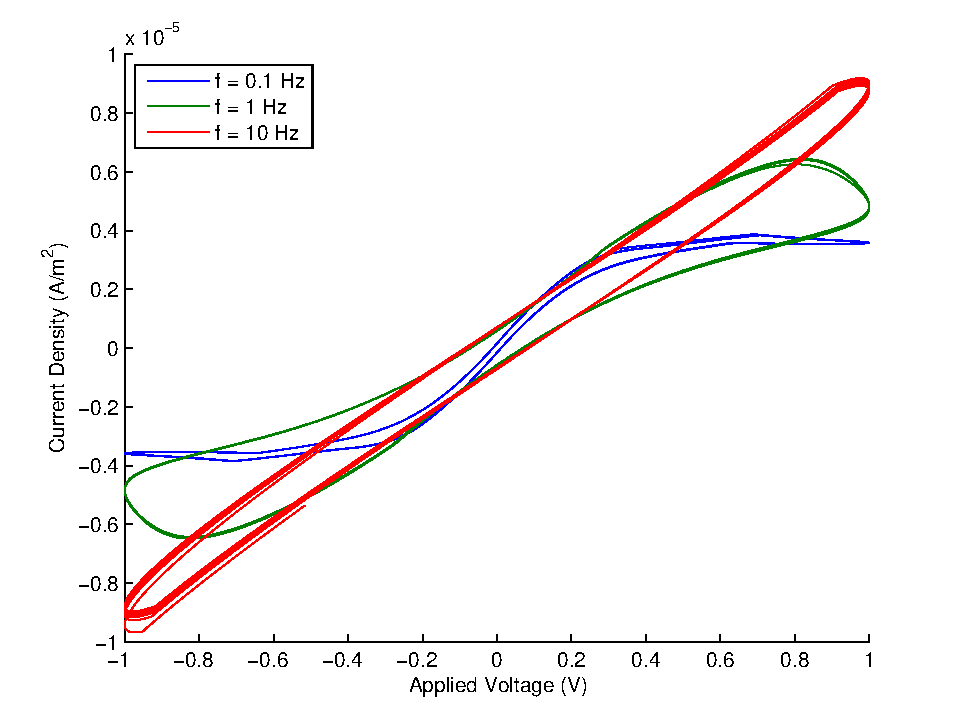
\includegraphics[scale=0.65]{MemF}
\caption{} 
\label{}
\end{figure}

\begin{figure}[!htp]
\centering
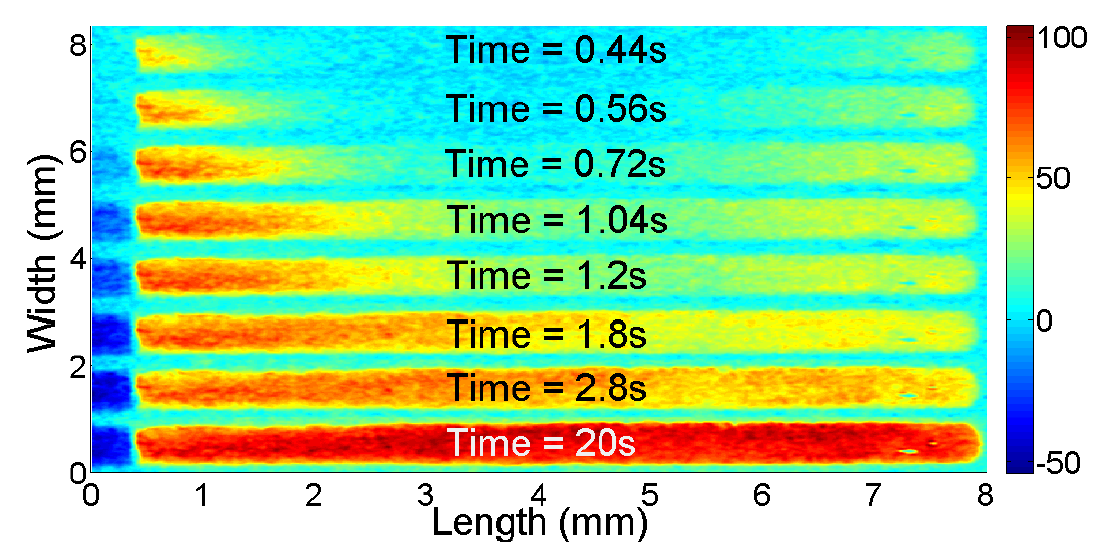
\includegraphics[scale=0.45]{notch}
\caption{} 
\label{}
\end{figure}

\begin{figure}[!htp]
\centering
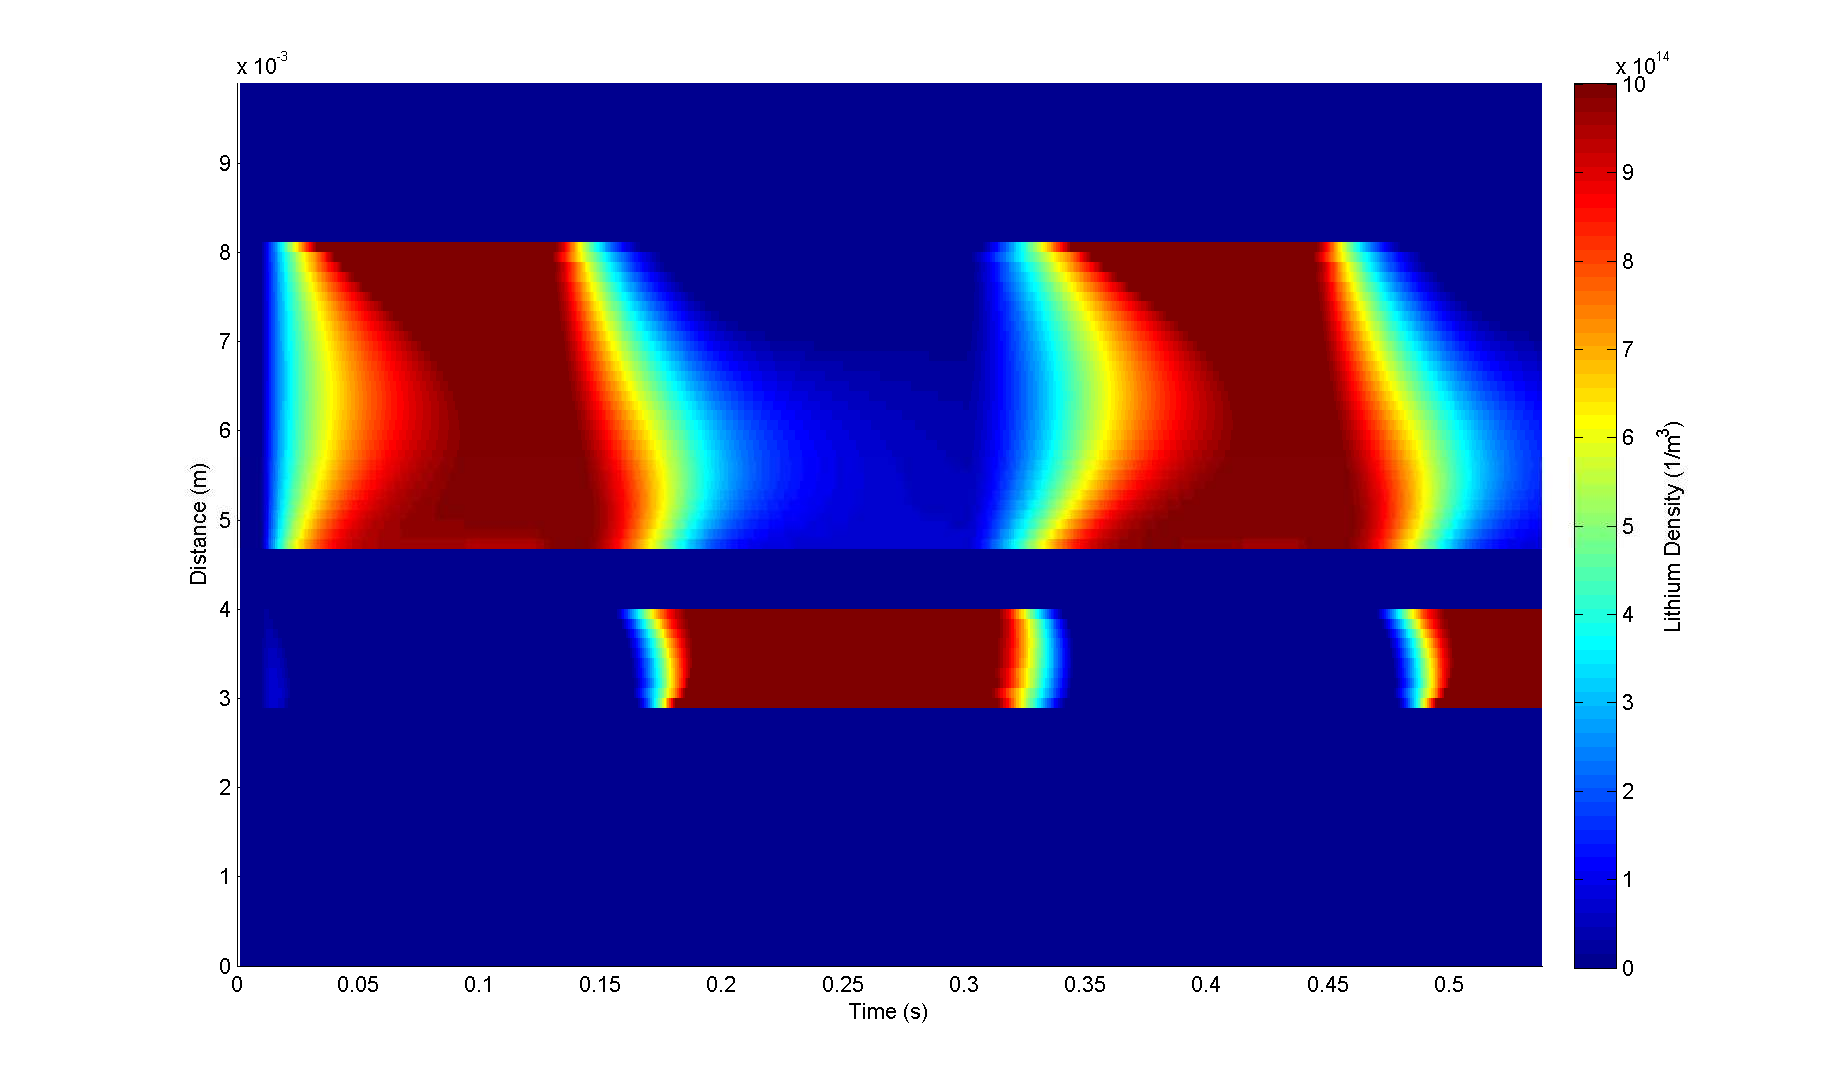
\includegraphics[scale=0.45]{Notch_flip_side}
\caption{} 
\label{}
\end{figure}
